\documentclass[10pt,fleqn,a4paper]{jsarticle}
\usepackage[dvipdfmx]{graphicx,color}
\usepackage{ascmac,amsmath,amssymb,amstext}
\usepackage{tikz,multicol,float,tikz-3dplot}
\usetikzlibrary{positioning,intersections,calc,arrows.meta,math,angles,patterns}
\usepackage{zogeny,ceo,comment}
\newcommand{\theme}[1]{【\text{#1}】}
\newcommand{\ans}[1]{\mbox{\boldmath{$#1$}}}
\renewcommand{\baselinestretch}{1.3} 
\newcommand{\hokusomu}[1]{
\begin{tikzpicture}[scale=1]
\filldraw[fill=black,draw=black](0,0)--({1-0.2},{0})--({1-0.2},{1-0.2})--(0,{1-0.2})--(0,0);
\draw[-,thick](0,0)--({1-0.2},{0})--({1/2-0.2},{1-0.2})--(0,{1-0.2})--(0,0);
\node[white,font=\Huge]at({1/2-0.1},{1/2-0.1})(label){$\mathbf{#1}$};
\end{tikzpicture}}
\newcommand{\hokukai}{
    \begin{tikzpicture}
  \draw[line width=0.2mm](-0.73,{-1/4+0.04})--(-0.73,{1/4-0.03})--(0.73,{1/4-0.03})--(0.73,{-1/4+0.04})--cycle;
  \draw[line width=0.6mm](-0.73,{-1/4+0.03})--(-0.73,{1/4-0.02});
  \draw[line width=0.6mm](0.73,{-1/4+0.03})--(0.73,{1/4-0.02});
  \node at(0,0){\kurosankakub \ans{解答}\kurosankakua};
\end{tikzpicture}
} %全国大学入試問題の「解答」記号
\tdplotsetmaincoords{60}{110}%{xy平面からどれだけ上にいるか(90度から-90度)}{z軸中心にどれだけ左右に回転するか}
\title{数学の核心-文理共通}
\author{大島　遙斗}
\begin{document}
\maketitle
\newpage
\tableofcontents
\newpage
{\Large \ans{はじめに}}\\
数学の勉強において一番大切なことは何でしょうか.\\\\
もしあなたが今,数学を勉強する上で一番大切なことは,「定理・公式を覚えて,1つ1つの問題の解き方を暗記すること.」
「難問は,解けなくても解法だけ暗記すれば良い.」などと思っているのであれば,今後数学の学力を向上していくのは難しいでしょう.\\\\
これは,私の高校1年生の時の体験です.高校1年生の時に私は,数学3までを青チャートで終わらせていました.ですが,模試などで結果が出ず原因
は何か真剣に考えました.愚かだった当時の私は,「演習量が足りないのだ!!」と考え,チャートを2周しました.結果は同じでした.\\\\
露頭に迷った私は,東進(対面授業をしている特別なコース)に足を運びます.そこで,一人の予備校の先生と出会います.青木純二先生です.青木先生(以下,青純)は,
授業の冒頭でいいました.\\\\
「ただ解法を暗記して,問題と解法を1対1に対応させているだけでは,いつまで経っても数学は強くならない.自然な発想で
試行錯誤しながら,当たり前と思える解法を発想できるようになることが超難関大を攻略する唯一の方法である.」\\\\
これだ!!と思いました.高校2年生の初めです.(第一期数学の真髄)そこからこの先生の授業を受け続け,数学は飛躍的に伸びていきました.高2の河合塾の全統記述
模試では,160/200をとりました.そこから,高3の秋に受けた河合塾の東工大オープンでは,220/300という驚異的な数字を叩き出すことができました.(確か全国80位)\\\\
このように従来の勉強方法では,成績は上がらないと確信しています.ですが,基本原理を身につけないで考えるとか大袈裟な事を言ってもしょうがないです.
このテキストでは,\ans{考える}ために必要な基本原理を徹底的に追求していきます.例えばいま,あなたが「軌跡を求めるときにパラメータを消去できるのはなぜか?」と
質問されて答えることができないならあなたは何もわかっていません.そこで,「パラメータが消去できる理由」「階差数列の公式はなぜ成り立つのか」「確率はなぜ掛け算できるのか」
「加法定理の証明」「ベクトルとは何か」etc...などさまざまなことを学習していきます.\\
1年後には,見違える数学の力がついているとお約束します.ぜひ一緒に頑張りましょう.\\
\hspace{13cm}大島　遙斗
\newpage
{\Large \ans{本書の使い方}}\\
講義形式です.\enpitu のところが学習する内容の重要事項です.そこを読んでから,問題を解いてきてください.問題は難しいものもあるので,解けなくても構いませんが
\ans{自分がどこまで考えたか？}は明確にしておいてください.とにかく,\ans{粘り強く考えること}が何より大切です.
\newpage
\section{差分の基礎}
数列における一番大事なことは？と人い問われたら,僕は,\ans{差分だね.}と答えます.数列を攻略する上で,差分はとても強力な武器になります.
\begin{itembox}
    [l]{\enpitu 差分の定義}
    $ある数列f(n)に対して,\Delta f(n)を\ans{差分列(階差数列)}と呼び,次のように定義する.$
    \begin{center}
        $\Delta f(n)=f(n+1)-f(n)$
    \end{center}
\end{itembox}
微分と積分が逆操作であるように,差分にも逆操作がありあます.それは,和をとることすなわち$\wa{}{}　計算です.$
\begin{itembox}
    [l]{\enpitu 和分の定義}
    $ある数列f(k)のn=1からn=kまでの和Sを求めるとき,f(k)の原始差分列(差分してf(k)になるような数列)がF(k)と分かっているとき,次の関係がある.$
    \begin{center}
        $S=\wa{k=1}{n}f(k)=\wa{k=1}{n}\Delta F(k)=\tint{F(k)}{1}{n+1}=F(n+1)-F(1)$
    \end{center}
\end{itembox}
微分と積分に線形性があるように差分と和分にも線形性(線形性:作用素が作用するのは,変数の部分だけ.つまり,定数は作用されない.)があります.
\begin{itembox}
    [l]{\enpitu 線形性}
    $\alpha,\beta を定数とする.$\\
    $\bullet 微分の線形性　\B{\alpha f(x)+\beta g(x)}^\prime=\alpha f^\prime(x)+\beta g^\prime(x)$\\
    $\bullet 積分の線形性　\dint{a}{b}\B{\alpha f(x)+\beta g(x)}dx=\alpha\dint{a}{b}f(x)dx=\beta\dint{a}{b}g(x)dx$\\
    $\bullet 差分の線形性　\Delta\B{\alpha f(k)+\beta g(k)}=\alpha\Delta f(k)+\beta\Delta g(k)$\\
    $\bullet 和分の線形性　\wa{k=1}{n}\B{\alpha f(k)+\beta g(k)}=\alpha\wa{k=1}{n}f(k)+\beta\wa{k=1}{n}g(k)$
\end{itembox}
\newpage
また,連続する整数の和にも美しい性質があります.
\begin{itembox}
    [l]{\enpitu 連続整数積の和の性質}
    \noindent\kakkoichi $\wa{k=1}{n}k=\tint{\dfrac{1}{2}k(k-1)}{k=1}{k=n+1}=\dfrac{1}{2}n(n+1)\\\\
    \kakkoni \wa{k=1}{n}k(k+1)=\tint{\dfrac{1}{3}(k-1)k(k+1)}{k=1}{k=n+1}=\dfrac{1}{3}n(n+1)(n+2)\\\\
    \kakkosan \wa{k=1}{n}k(k+1)(k+2)=\tint{\dfrac{1}{4}(k-1)k(k+1)(k+2)}{k=1}{k=n+1}=\dfrac{1}{4}n(n+1)(n+2)(n+3)$
\end{itembox}
では,問題を解いてみましょう.\\
\newpage
\noindent\ba{1$\bullet$1}.$以下の数列の差分列\Delta f(k)を求めよ.$\\
\kakkoichi $f(k)=k$\\
\kakkoni $f(k)=k^2\\
\kakkosan f(k)=k^3\\
\kakkoshi f(k)=k(k+1)(k+2)(k+3)\\
\kakkogo f(k)=2^k\\
\kakkoroku f(k)=3^k\cdot k^2\\
\kakkoshichi f(k)=\dfrac{1}{k!}\\
\kakkohachi f(k)=5\\
\kakkokyu f(k)=0$\\\\
\ba{1$\bullet$2}.$以下の数列の和を\ans{和差分の関係を用いて}それぞれ求めよ.$\\
\kakkoichi $A_n=\wa{k=1}{n}1\\
\kakkoni B_n=\wa{k=1}{n}k\\
\kakkosan C_n=\wa{k=1}{n}k^2\\
\kakkoshi D_n=\wa{k=1}{n}k^3\\
\kakkogo E_n=\wa{k=0}{n^2+1}k(k+1)(k+2)(k+3)\\
\kakkoroku F_n=\wa{k=-3}{n-1}(k+2)(k+3)(k+4)^2\\
\kakkoshichi G_n=\wa{k=1}{n}2^k\\
\kakkohachi H_n=\wa{k=1}{n}(k+2)\cdot3^k\\
\kakkokyu I_n=\wa{k=1}{n}k^4$\\\\
\ba{1$\bullet$3}.次の和を求めよ.\\
\kakkoichi$\wa{k=1}{n}\B{\p{k+1}^7-k^7}$\\
\kakkoni$\wa{k=1}{n}\dfrac{1}{\sqrt{k+1}+\sqrt{k}}$\\
\kakkosan$\wa{k=1}{n}\dfrac{1}{k(k+1)}$
\newpage
\begin{center}
    \large{\ans{1章の問題演習}}
\end{center}
\reibanichi 　$nを自然数とする.次の和を求めよ.\\
\kakkoichi A_n=\wa{k=2}{n}\dfrac{1}{k(k-1)}\hspace{3cm}\kakkoni B_n=\wa{k=1}{n}\dfrac{1}{k(k+1)(k+2)}\\
\kakkosan C_n=\wa{k=1}{n}k(k+1)\hspace{3cm}\kakkoshi D_n=\wa{k=-3}{n}(k+2)(k+3)(k+4)\\
\kakkogo E_n=\wa{k=0}{n}(n-k)(n-k+1)(n-k+2)$
\newpage
\section{差分の応用}
前回学習した差分を使って,高校数学\suB を整理し直します.ここで,皆さん覚えろと指示された等差数列・等比数列の公式覚えるまでもない一瞬で導ける,当たり前な概念へと昇華させます.\\
お楽しみに.\\\\
まずは,差分と和分の復習です.
\begin{itembox}
    [l]{\reidaic }
    次の数列の差分列を求めよ.
\begin{align*}
    f(k)=r^k　(r>0)
\end{align*}
\end{itembox}
\kai\\
$\Delta f(k)=r^{k+1}-r^k=\ans{(r-1)\cdot r^k}$\\\\
余裕ですね.それでは,お次は和分です.\\
\begin{itembox}
    [l]{\reidaic}
    次の数列の和を差分を用いて求めよ.
    \begin{align*}
        S_n=\wa{k=1}{n}r^{k}　(r>0)
    \end{align*}
\end{itembox}
\kai\\
まず,$g(k)=r^kとおいて,差分してg(k)になるような数列(原始数列):G(k)を見つける.$
\begin{align*}
    \Delta g(k)=(r-1)\cdot r^k\doti r^k=\Delta\B{\dfrac{g(k)}{r-1}}=\Delta\B{\dfrac{r^k}{r-1}}　(\because 差分の線形性)
\end{align*}
従って,$G(k)は$
\begin{align*}
    G(k)=\dfrac{r^k}{r-1}\hspace{2mm}である.
\end{align*}
これより,$S_n$は,
\begin{align*}
    S_n=\wa{k=1}{n}\Delta\B{\dfrac{r^k}{r-1}}&=\tint{\dfrac{r^k}{r-1}}{k=0}{k=n+1}\\
    &=\ans{\dfrac{r^{n+1}-1}{r-1}=\dfrac{1-r^{n+1}}{1-r}}　\p{\temarkua \dfrac{(最後の次)-(最初)}{(公比)-1}=\dfrac{(最初)-(最後の次)}{1-(公比)}}
\end{align*}
\newpage
\noindent これで,等比数列の和の公式が導かれました.慣れるまでは,\ans{必ず}自分で導いて使うようにしてください.慣れたら,覚えてください.
\begin{itembox}
    [l]{\enpitu 等比数列の和公式}
    等比数列$a_n=r^n　(r>0)$に対して,初項から第$n項$までの和$S_n$は次の形で表せる.
    \begin{center}
        $S_n=\wa{k=1}{n}r^k=\ans{\dfrac{r^{n+1}-1}{r-1}}=\ans{\dfrac{1-r^{n+1}}{1-r}}$
    \end{center}
    覚え方は,$\ans{\dfrac{(最後の次)-(最初)}{(公比)-1}},または,\ans{\dfrac{(最初)-(最後の次)}{1-(公比)}}$である.
\end{itembox}\\
次に等差数列について考えます.
\begin{itembox}
[l]{\enpitu 等差数列の定義}
\noindent・等差数列$\cdots$前後の項において,\ans{「ある一定の差」}を規則に持つような数列.
\end{itembox}
（例）\begin{align*}
    a_1\xrightarrow{+d}a_2\xrightarrow{+d}a_3\xrightarrow{+d}\cdots\xrightarrow{+d}a_n　(\temarkua 等差　+dは一定の差)\\
\end{align*}
これって,中学校で習う\ans{一次関数の振る舞い}に似ていませんか？次のような感じ.
\begin{center}
    \begin{tikzpicture}
        \draw[->,>=Latex](-1.5,0)--(6,0)node[right]{$n(項番号)$};
        \draw[->,>=Latex](0,-1.5)--(0,6)node[above]{$y(項の値)$};
        \begin{scope}
            \clip(-1.5,-1.5)rectangle(6,6);
            \draw[thin] plot(\x,{\x+1});
            \node[above left]at(4,5){$y=a_n+d$};
            \node[below left]at(0,0){O};

            \draw[dashed](1,0)--(1,2)--(0,2)node[left]{$a_2$};
            \node[below]at(1,0){2};
            \filldraw[fill=black,draw=black](1,2)circle(2pt);

            \draw[dashed](2,0)--(2,3)--(0,3)node[left]{$a_3$};
            \node[below]at(2,0){3};
            \filldraw[black](2,3)circle(2pt);
            \draw[->,>=Latex,thick](1,2)--(2,2) node[midway,below]{$+1$};
            \draw[->,>=Latex, thick](2,2)--(2,3) node[midway,right]{$a_2+d$};
            \draw[ultra thick](1,2)--(2,3);
            \draw[thin] (1.5,{1.5+1}) to[out=120,in=200] (1.55,3.5);
            \node[above] at (1.55,3.5) {傾き($d$)};
        \end{scope}
    \end{tikzpicture}
\end{center}
つまり,\ans{等差数列は,一次関数と同様に扱える.}ということが言えます.\\また,\ans{「傾き」は「数列の公差」},\ans{「面積」は「数列の和」}に対応します.
このことから等差数列の種々の公式を導きましょう.
\newpage
\noindent 等差数列と一次関数の対応関係について, 抑えておきましょう.
\begin{align*}
    &\bullet 「傾き」は,\ans{「公差」}に.\\
    &\bullet 「直線の方程式」は,\ans{「一般項」}に.\\
    &\bullet 「面積」は,\ans{「総和」}に.
\end{align*}
それぞれ対応する.\\
このことを用いて次の例題を解きましょう.\\
\reidaic　 $p,qはp<qを満たす自然数とする.このとき,以下の問に答えよ.$\\
\kakkoichi\hspace{2mm}$第p項がA,第q項がBであるような等差数列\B{a_n}の一般項をp,q,A,B,nで表せ.また,この数列の第p項から第q項までの和Sをp,q,A,Bで表せ.$\\
\kakkoni\hspace{2mm}$第p項がC,第q項がD\hspace{2mm}(ただし,C>0,D>0,C\neq D)であるような公比が正の等比数列\B{b_n}について,x=\dfrac{1}{q-p}とおくとき,
\B{b_n}の第p項から第q項までの和TをC,D,xで表せ.$
\noindent\kangaekata\\
\kakkoichi 等差数列のグラフを描いて,直線の方程式を求めれば一般項はでます.和は,$qからpまでの面積を求めれば良いです$.\\
\kakkoni 「よくわからない数列の和は書き下す.」という原則に従いましょう.\\
\kai\\
\kakkoichib 等差数列のグラフは下図のようになっている.
\begin{center}
    \begin{tikzpicture}
        \draw[->,>=Latex](-1,0)--(5,0)node[right]{$n(項番号)$};
        \draw[->,>=Latex](0,-1)--(0,5)node[above]{$y(項の値)$};
        \begin{scope}
            \clip(-0.5,-0.5)rectangle(5,5);
            \draw[thin] plot(\x,{\x+1});
            \draw[dashed](1,0)--(1,2)--(0,2)node[left]{$A$};
            \node[below]at(1,0){$p$};
            \draw[dashed](3,0)--(3,4)--(0,4)node[left]{$B$};
            \node[below]at(3,0){$q$};
            \fill[black!20](1,0)--(1,2)--(3,4)--(3,0)--(1,0);
            \draw[very thick](1,0)--(1,2)--(3,4)--(3,0)--(1,0);
            \node[below left]at(0,0){O};
        \end{scope}
    \end{tikzpicture}
\end{center}
上図より,等差数列の一般項は直線の方程式なので,傾き$\dfrac{B-A}{q-p}より,$
\begin{align*}
    \ans{a_n=\dfrac{B-A}{q-p}\p{n-p}+A}
\end{align*}
また,$qからp$までの面積は,上図の網目部に対応するので,台形の面積の公式より,
\begin{align*}
    \ans{S=\dfrac{1}{2}\p{q-p+1}\p{B+A}}
\end{align*}
\kakkonib
与えられた等比数列の構造は,下表のようになっている.
 \begin{center}
    \begin{tabular}{c||ccccccccc}
        $n$ & 1& 2 & 3 & $\cdots$ & $p$ & $\cdots$ & $q$ & $\cdots$ & $n$\\
        \hline
        $a_n$ & $a_1$ & $a_2$ & $a_3$ & $\cdots$ & $C$ & $\cdots$ & $D$ & $\cdots$ & $a_n$
    \end{tabular}
\end{center}
表より,公比は$\dfrac{D}{C}であり,Tは第p項から第q項までに公比をq-p回かければ良いので,求める和Tは$
\begin{align*}
    T&=C+C\cdot\dfrac{D}{C}+\cdots+C\cdot\p{\dfrac{D}{C}}^{q-p}\\
    &=C\cdot\wa{k=p}{q}\p{\dfrac{D}{C}}^{k}=C\cdot\wa{k=p}{q}r^{k}　\p{r=\dfrac{D}{C}とおいた.}\\
    &=C\cdot\dfrac{1-r^{q-p+1}}{1-r}=\ans{C\cdot\dfrac{1-\p{\frac{D}{C}}^{\frac{1}{x}+1}}{1-\frac{D}{C}}}
\end{align*}\\
関数の増加と減少を微分と増減表により調べるように,数列の増減も差分列により判断することができます.
\begin{itembox}
    [l]{\enpitu 数列の増加・減少の差分による判断}
    $ある数列f(k)を考える.\\
    \bullet\hspace{2mm} \Delta f(k)=f(k+1)-f(k)>0\doti f(k)は増加数列.\\
    \bullet\hspace{2mm}\Delta f(k)=f(k+1)-f(k)=0\doti f(k)は定数数列.\\
    \bullet\hspace{2mm}\Delta f(k)=f(k+1)-f(k)<0\doti f(k)は減少数列.$
\end{itembox}
\newpage
\noindent\ba{2$\bullet$1}次の和を求めよ.\\
\kakkoichi $A_n=\wa{k=-n}{n}3^k$\\
\kakkoni $B_n=\wa{k=1}{n}\dfrac{k}{2^k}$\\
\kakkosan $C_n=\wa{k=1}{n}k^2\cdot3^k$\\\\
\ba{2$\bullet$2}\\
次の$f(n)を最大にする自然数nを求めよ.$
\begin{align*}
    f(n)=n\p{\dfrac{20}{21}}^n
\end{align*}\\
\ba{2$\bullet$3}\\
$4以上のすべての自然数nに対して,2^n\geq n^2が成り立つことを証明せよ.$
\newpage
\begin{center}
    \ans{2章の問題演習}
\end{center}
\reibanichi　$nを自然数とする.次の和を求めよ.$
\begin{align*}
    &\kakkoichi F_n=\wa{k=1}{n}3^k &\kakkoni G_n=\wa{k=-n}{n}2^k\\
    &\kakkosan H_n=\wa{k=0}{n}\dfrac{2^{2k-1}}{3^{k+2}}&\kakkoshi I_n=\wa{k=1}{n}k\cdot3^k\\
    &\kakkogo J_n=\wa{k=1}{n}k(k+1)(k+5)\cdot2^k &\kakkoroku K_n=\wa{k=1}{n}k\cdot k!  
\end{align*}\\
\reibanni　$nが2以上の整数のとき,次の不等式が成り立つことを証明せよ.$
\begin{align*}
    \dfrac{1}{1^2}+\dfrac{1}{2^2}+\dfrac{1}{3^2}+\cdots+\dfrac{1}{n^2}<2-\dfrac{1}{n}
\end{align*}\\
\reibansan　不等式
\begin{align*}
    5^n<2^n\cdot n(n+2)
\end{align*}
を満たす自然数$n$を全て求めよ.
\newpage
\section{漸化式}
今回は,基本的な漸化式を扱います.苦手な人が多い理由はそれぞれの漸化式の解き方を覚えているからにすぎません.漸化式は実は,\ans{3つの基本漸化式に帰着させる}
ことでしか解くことができないのです.\\その3つとは,\ans{\doichi.等差型,\doni.等比型.\dosan.階差(差分)型}です.\\\\
$以下,n\in\mathbb{N}とします.$
\begin{itembox}
[l]{\enpitu \doichi.等差型漸化式}
$dを定数として,次の形の漸化式を等差型漸化式と呼ぶ.$
\begin{center}
    $a_{n+1}=a_n+d$
\end{center}
さらにその一般項$\B{a_n}は,$
\begin{center}
    $\ans{a_n=a_1+(n-1)d}$
\end{center}
で表される.
\end{itembox}
\begin{itembox}
    [l]{\enpitu\doni. 等比型漸化式}
    $rを定数として,次の形の漸化式を等比型漸化式と呼ぶ.$
    \begin{center}
        $a_{n+1}=ra_n$
    \end{center}
また,この数列の構造は以下のようになっている.
\begin{center}
    $a_1\xrightarrow{\times r}a_2\xrightarrow{\times r}a_3\xrightarrow{\times r}\cdots\xrightarrow{\times r}a_n$
\end{center}
したがって,$\ans{a_1にrを(n-1)回かければa_nになる}ので,その一般項\B{a_n}は,$
\begin{center}
    $\ans{a_n=a_1\cdot r^{n-1}}$
\end{center}
で表される.
\end{itembox}
\begin{itembox}
    [l]{\enpitu \dosan.階差型(差分型)漸化式}
    $f(n)をある規則を持った数列として,次の形の漸化式を階差型(差分型)漸化式と呼ぶ.$
    \begin{center}
        $a_{n+1}=a_n+f(n)$
    \end{center}
    また,この数列の構造は以下のようになっている.
    \begin{center}
        $a_1\xrightarrow{+f(1)}a_2\xrightarrow{+f(2)}a_3\xrightarrow{+f(3)}\cdots\xrightarrow{+f(n-1)}a_n$
    \end{center}
したがって,$a_1+f(1)+f(2)+f(3)+\cdots+f(n-1)=a_1+\wa{k=1}{n-1}f(k)=a_nになるので,その一般項\B{a_n}は$
\begin{center}
    $\ans{n\geq2のとき,a_n=a_1+\wa{k=1}{n-1}f(k)}$
\end{center}
と表される.また,$n=1のときに上式は成立しないので,n=1のときのa_nの成立も確認しなければならない.$
\end{itembox}\\
世の中の漸化式(力学系などの数学3の範囲・カオス的な漸化式を除く)は全てこの三つの漸化式に帰着させて解きます.\\
なので,皆さん覚えがちな次の形をした漸化式を2通りの方法で解いてみましょう.(次ページ)\\\\
\newpage
$\noindent\bullet \doshi \ans{応用型漸化式}\\
pを定数として次の形の漸化式を応用型漸化式とよぶ.$
\begin{center}
    $a_{n+1}=pa_n+f(n)\cdots\cdots\cdots\asta$
\end{center}
そして,解き方は,\kuromaruichi 「階差型への帰着」と\kuromaruni 「等比型への帰着」の二つがある.まず,\kuromaruichi をみてみよう.\\
\kuromaruichi\underline{\ans{階差型への帰着}}\\
\kangaekata\\
$\asta のpがなかったら,階差型になる!じゃあ,\asta の両辺をp^nかp^{n+1}で割ってみよう!$\\
\kai\\
$\asta の両辺をp^{n+1}で割ると,$
\begin{align*}
    \dfrac{a_{n+1}}{p^{n+1}}=\dfrac{a_n}{p^n}+\dfrac{f(n)}{p^{n+1}}
\end{align*}
$b_n=\dfrac{a_n}{p^n}とおけば,b_{n+1}=b_n+\dfrac{f(n)}{p^{n+1}}となってこれは,階差型の漸化式である.$\\\\
これで,目標が達成できました.つぎに\kuromaruni へ行きたいところですが,\ans{特性方程式}を使うので,皆さん訳わからずにつかっている
特性方程式について,注意,モチベージョンを話しておきます.\\
\fbox{\chud 特性方程式について.}\\
特性方程式とは,その方程式(漸化式とか微分方程式とか)を満たすような数列ないし関数をテキトーに予想して,それを計算することで一般の
式に対する特殊解を探すような方程式である.すなわち,\ans{実験しないと特殊解は見つからない.}ということである.だが,その特殊解
は先人の努力により分かっている.次のようなことが知られている.\\
$\ans{1.a_{n+1}=pa_n+f(n)型}\to 定数数列が特殊解.\\
\ans{2.a_{n+2}=pa_{n+1}+qa_n型}\to 等比数列が特殊解.$\\
そのため,$a_{n+1}=pa_n+f(n)の漸化式は,\ans{\alpha=p\alpha+f(n)}という特性方程式を解くのである.\\
同様に,隣接三項間型漸化式:a_{n+2}=pa_{n+1}+qa_nは,\ans{\alpha^2=p\alpha+q}という特性方程式を解くのである.\ans{(注意終わり)}$\\\\
\kuromaruni\underline{\ans{等比型への帰着}}\\
\kangaekata\\
$\asta のf(n)がなかったら,等比型になるな.じゃあ,\asta を満たす数列を一つ見つけて,引き算すればf(n)消えるやん.とりあえず,
定数数列:b_n=\alpha みたいな数列が\asta をみたすか実験してみよう!　\alpha=p\alpha+f(n)になって,\asta を満たすぞ!$\\\\
\kai\\
引き算すると,$a_{n+1}-d=p\p{a_n-d}となって,これは等比型漸化式で目標は達成.$\\
では,次の問題を5分を目安に2つの解法で解いてみてください.\\
\fbox{$a_1=6,a_{n+1}=4a_n-3\cdots\bigstar(n=1,2,3,\cdots)の一般項を求めよ.$}\\
\kuromaruichi \underline{階差型への帰着.}\\
\kai\\
$\bigstar の両辺を4^{n}で割ると,$
\begin{align*}
    \dfrac{a_{n+1}}{4^n}=\dfrac{a_n}{4^{n-1}}-\dfrac{3}{4^n}
\end{align*}
これより,$n\geq2のとき,$
\begin{align*}
    \dfrac{a_n}{4^{n-1}}&=a_1-3\wa{k=1}{n-1}\dfrac{1}{4^n}\\
    &=6-3\cdot\dfrac{\frac{1}{4}-\frac{1}{4^n}}{1-\frac{1}{4}}\\
    &=5+\dfrac{1}{4^{n-1}}
\end{align*}
$\yueni a_n=5\cdot4^{n-1}+1で,これは,n=1のときも成立するから,求める一般項は,\ans{a_n=5\cdot4^{n-1}+1(n\geq1)}$\\
\kuromaruni\underline{等比型への帰着.}\\
\kai\\
$a_n=\alpha が\bigstar を満たすとすると,$
\begin{align*}
    \alpha=4\alpha-3\doti \alpha=1
\end{align*}
これより,$a_n=1は\bigstar を満たす特殊解である.すなわち,1=4\cdot1-3を満たすので,これを\bigstar から辺々引くと,$
\begin{align*}
    a_{n+1}-1=4\p{a_n-1}(n\geq1)
\end{align*}
となり,これは,$初項(a_1-1)=5の等比数列である.$\\
よって求める一般項は,$1a_n-1=5\cdot4^{n-1}\doti\ans{a_n=5\cdot4^{n-1}+1(n\geq1)}$\\\\
必ず,どっちでも解けるようにしましょう.\\
次に,隣接三項間型漸化式です.(次ページ)
\newpage
$\noindent\bullet\dogo\ans{隣接三項間型漸化式}$\\
$p,qを定数として,次の形の漸化式を隣接三項間型漸化式と呼ぶ.$
\begin{center}
    $a_{n+2}=pa_{n+1}+qa_n\cdots\asta$
\end{center}
そして,解き方は,\kuromaruichi 「等比型への帰着(教科書を見よ)」と\kuromaruni 「線形結合を利用し一般解を表す方法」の二つがある.
\kuromaruichi は教科書ないし参考書をみよ.\kuromaruni の解き方を述べる前に,\ans{線形結合とは？}を解説する.\\\\
\fbox{\chud 線形結合とは？}\\
今考えている方程式のrank(次数)が$n(n次)のとき,\alpha_1,\alpha_2,\cdots,\alpha_mのm個の特殊解が得られており,定数C_1,C_2,C_3,\cdots C_mとして,一般解(一般項)は次のように表すことができる.$
\begin{center}
    $a_n=\wa{k=1}{m}\alpha_k\cdot C_k=\alpha_1\cdot C_1+\alpha_2\cdot C_2+\cdots+\alpha_m\cdot C_m$
\end{center}
そして,$m個の定数は初期条件(a_1,a_2,\cdots,a_mの値)から連立方程式を解くことにより求めることができ,その結果が一般解である.\ans{(注意終わり)}$\\\\
\kuromaruni \underline{線形結合を利用し一般解を表す方法.}\\
\kai\\
$a_n=r^{n-1}が\asta を満たすとすると,\asta に代入して$
\begin{align*}
    r^{n+1}=pr^n+qr^{n-1}&\doti r^{n-1}\p{r^2-pr-q}=0\\
    &\doti r^2-pr-q=0\\
    &\doti \p{r-\alpha_1}\p{r-\alpha_2}=0\p{\temarkua 一時的にr=\alpha_1,\alpha_2が解と仮定した.}\\
    &\doti a_n=\alpha_1^{n-1},\alpha_2^{n-1}は\asta を満たす特殊解.
\end{align*}
これより,定数を$C_1,C_2として\asta の一般項は,$
\begin{center}
    $a_n=C_1\cdot\alpha_1^{n-1}+C_2\cdot\alpha_2^{n-1}$
\end{center}
と表すことができる.あとは,初期条件より,定数を定めれば良い.簡単でしょ??\\
では,この方法で次の問題を5分を目安に解いてみてください.\\
\fbox{$a_1=0,a_2=1,a_{n+2}=a_{n+1}+6a_n\cdots\bigstar(n=1,2,3,\cdots)の一般項を求めよ.$}
\newpage
\noindent\kai\\
$a_n=x^{n-1}が\bigstar を満たすとすると,代入するこにより,$
\begin{align*}
    x^{n+1}=x^n+6x^{n-1}&\doti x^{n-1}\p{x^2-x-6}=0\\
    &\doti (x-3)(x+2)=0\\
    &\doti x=3,-2
\end{align*}
よって,$a_n=3^{n-1},\p{-2}^{n-1}は\bigstar を満たす特殊解である.これより,定数をC_1,C_2とおくと,一般項\B{a_n}は$
\begin{align*}
    a_n=C_1\cdot3^{n-1}+C_2\cdot\p{-2}^{n-1}\cdots\cdots\cdots\maruichi 
\end{align*}
と表せる.初期条件から,
\begin{align*}
    \begin{cases}
        0=C_1+C_2\\
        1=3C_1-2C_2
    \end{cases}&\doti\begin{cases}
    C_1=-C_2\\
    1=3C_1+2C_2
    \end{cases}\doti\begin{cases}
        C_1=\frac{1}{5}\\
        C_2=-\frac{1}{5}
    \end{cases}
\end{align*}
$\Y 求める一般項は,\ans{a_n=\dfrac{1}{5}\p{3^{n-1}-\p{-2}^{n-1}}\p{n\geq1}}$\\\\
では,次に,\ans{特殊解が1つしか得られなかった場合の一般項の求め方}について説明します.\\
次の性質は,認めてください.
\begin{itembox}
    [l]{\chud 特殊解が重解の場合と線形結合}
    今,$隣接三項間型漸化式の特殊解が,a_n=r^{n-1}と一つしか得られなかったとする.このとき,一般項\B{a_n}は,$
    \begin{center}
        $a_n=C_1\cdot r^{n-1}+C_2\cdot n\cdot r^{n-1}$
    \end{center}
    と表すことができる.\\
    つまり,もう一つの特殊解は,$\ans{得られた特殊解のn倍である.}ということです.$
\end{itembox}
では,次の問題も同様に5分を目安に解いてみてください.\\
\fbox{$a_1=2,a_2=3,a_{n+2}-4a_{n+1}+4a_n=0\cdots\bigstar(n=1,2,3,\cdots)の一般項を求めよ.$}
\newpage
\noindent\kai\\
$a_n=x^{n-1}が\bigstar を満たすとすると,代入することにより,$
\begin{align*}
    x^2-4x+4=0&\doti (x-2)^2=0\\
    &\doti x=2
\end{align*}
よって,$a_n=2^{n-1},n\cdot2^{n-1}は\bigstar を満たす特殊解である.これより,定数をC_1,C_2とおくと,一般項\B{a_n}は,$
\begin{align*}
    a_n=C_1\cdot2^{n-1}+C_2\cdot n\cdot2^{n-1}\cdots\cdots\cdots\maruichi 
\end{align*}
と表せる.初期条件から,
\begin{align*}
    \begin{cases}
    2=C_1+C_2\\
    3=2C_1+4C_2
    \end{cases}&\doti\begin{cases}
        2C_1+2C_2=4\\
        2C_1+4C_2=3
    \end{cases}
    \doti\begin{cases}
        C_1=\frac{5}{2}\\
        C_2=-\frac{1}{2}
    \end{cases}
\end{align*}
$\Y 求める一般項は,\ans{a_n=\dfrac{5}{2}\cdot2^{n-1}-\dfrac{1}{2}\cdot n\cdot2^{n-1}(n\geq1)}$\\\\
重解の場合も簡単ですね!とかく,隣接三項間型漸化式にびびる必要はもうありません.\\
では,続いて連立漸化式についてみてゆくことにいたしましょう.
\newpage
\noindent$\bullet\doroku\ans{連立漸化式}$\\
$p,q,r,sを定数として,値が一致する場合も含めて次の形の漸化式を連立漸化式と呼ぶ.$
\begin{center}
    $\begin{cases}
        a_{n+1}=pa_n+qb_n\cdots\cdots\cdots\maruichi\\
        b_{n+1}=ra_n+sb_n\cdots\cdots\cdots\maruni
    \end{cases}(n\geq1)$
\end{center}
解き方は様々あるが,基本的に\kuromaruichi 「等比型への帰着」,\kuromaruni 「隣接三項間型への帰着」や\kuromarusan 「辺々足して等比型(係数が対称の場合)」がある.
\kuromaruni,\kuromarusan は簡単なので,省略する.\kuromaruichi について解説する.\\\\
\kuromaruichi\underline{等比型に帰着させる方法}\\
\kangaekata\\
$\maruichi,\maruni が等比型になるための条件は,\ans{\maruichi\times\alpha+\maruni\times\beta の係数比が等しくなること.}です.$\\
\kai\\
$\maruichi\times\alpha+\maruni\times\beta より,等比型に帰着するための条件は,$
\begin{align*}
    \alpha a_{n+1}+\beta b_{n+1}=\p{p\alpha+r\beta}a_n+\p{q\alpha+s\beta}b_n
\end{align*}
の係数比がそれぞれ等しくなることである.\\
したがって,
\begin{align*}
    \alpha:\beta=p\alpha+r\beta:q\alpha+s\beta&\doti p\alpha\beta+r\beta^2=q\alpha^2+s\alpha\beta\\
    &\doti q\alpha^2+(s-p)\alpha\beta-r\beta^2=0　(\temarkua 解けますね!)\\
    &\doti \cdots
\end{align*}
あとはこれを計算して係数比を出せば,等比型に帰着させることができるというワケです.\\
では,次の2題を合わせて15分を目安に取り組んでみてください.\\
\reibanichi$a_1=1,b_1=-1,\begin{cases}
    a_{n+1}=5a_n-4b_n\cdots\cdots\cdots\maruichi\\
    b_{n+1}=a_n+b_n\cdots\cdots\cdots\maruni
\end{cases}(n\geq1)$\\\\
\reibanni$a_1=b_1=1,　　\begin{cases}
    a_{n+1}=a_n+4b_n\cdots\cdots\cdots\maruichi\\
    b_{n+1}=a_n+b_n\cdots\cdots\cdots\maruni
\end{cases}(n\geq1)$
\newpage
\noindent\reibanichi\\
\kai
\begin{align*}
&\maruichi\times\alpha+\maruni\times\beta が等比型になる.\\
&\doti \alpha a_{n+1}+\beta b_{n+1}=(5\alpha+\beta)a_n+(-4\alpha+\beta)b_n の係数比がそれぞれ等しい.\\
&\doti \alpha:\beta=5\alpha+\beta:-4\alpha+\beta\\
&\doti 4\alpha^2+4\alpha\beta+\beta^2=0\\
&\doti \p{2\alpha+\beta}^2=0\\
&\doti \alpha:\beta=1:-2
\end{align*}
これより,
\begin{align*}
    a_{n+1}-2b_{n+1}=3\p{a_n-2b_n}&\doti a_n-2b_n=3^{n-1}\p{a_1-2b_1}=3^n\\
    &\doti a_n-2b_n=3^n\cdots\cdots\cdots\marusan
\end{align*}
$\marusan を\maruni に代入すると,$
\begin{align*}
    b_{n+1}=3b_n+3^n&\doti \dfrac{b_{n+1}}{3^n}=\dfrac{b_n}{3^{n-1}}+1\\
    &\doti \dfrac{b_n}{3^{n-1}}=\dfrac{b_1}{3^0}+\wa{k=1}{n-1}1=n-2　(n\geq2)\\
    &\doti b_n=3^{n-1}(n-2)
\end{align*}
これは,$n=1のときも成立する.$\\
$また,a_n=3^n+2b_nより,$
\begin{align*}
    a_n=3^{n-1}(2n-1)
\end{align*}
$\Y 以上より,求める一般項は,\ans{\begin{cases}
    a_n=3^{n-1}(2n-1)\\
    b_n=3^{n-1}(n-2)
\end{cases}(n\geq1)}$
\newpage
\noindent\reibanni\\
\kai
\begin{align*}
    &\maruichi\times\alpha+\maruni\times\beta が等比型になる.\\
    &\doti  \alpha a_{n+1}+\beta b_{n+1}=(\alpha+\beta)a_n+(4\alpha+\beta)b_nの係数比がそれぞれ等しい.\\
    &\doti \alpha:\beta=\alpha+\beta:4\alpha+\beta\\
    &\doti 4\alpha^2-\beta^2=0\\
    &\doti(2\alpha-\beta)(2\alpha+\beta)=0\\
    &\doti \alpha:\beta=1:2=1:-2
\end{align*}
$\bullet\hspace{2mm}\alpha:\beta=1:2より,\\
　a_{n+1}+2b_{n+1}=3(a_n+2b_n)\doti a_n+2b_n=(a_1+2b_1)\cdot3^{n-1}=3^n\cdots\cdots\cdots\marusan $\\
$\bullet\hspace{2mm}\alpha:\beta=1:-2より,\\$
　$a_{n+1}-2b_{n+1}=-(a_n-2b_n)\doti a_n-2b_n=(-1)^{n-1}(a_1-2b_1)=(-1)^n\cdots\cdots\cdots\marushi$\\\\
$\dfrac{\marusan+\marushi}{2}より,$
\begin{align*}
    a_n=\dfrac{3^n+(-1)^n}{2}
\end{align*}
$\dfrac{\marusan-\marushi}{4}より,$
\begin{align*}
    b_n=\dfrac{3^n-(-1)^n}{4}
\end{align*}
$\Y 求める一般項は,\ans{\begin{cases}
    a_n=\dfrac{3^n+(-1)^n}{2}\\
    b_n=\dfrac{3^n-(-1)^n}{4}
\end{cases}(n\geq1)}$
\newpage
\noindent\ba{3$\bullet$1}次の漸化式の一般項を求めよ.\\
\kakkoichi $a_1=2,a_{n+1}=3a_n　(n\geq1)$\\
\kakkoni $a_2=2,a_{n+1}=3a_n　(n\geq0)$\\
\kakkosan $a_1=2,a_n=3a_{n-1}　(n\geq1)$\\
\kakkoshi $a_2=2,a_{n+2}=3a_{n+1}　(n\geq1)$\\\\
\ba{3$\bullet$2}次の漸化式の一般項を階差型に帰着して求めよ.\\
\kakkoichi $a_1=1,a_{n+1}=2a_n+2^n　(n\geq1)$\\
\kakkoni $a_1=1,a_{n+1}=4a_n-6　(n\geq1)$\\\\
\ba{3$\bullet$3}次の漸化式の一般項を等比型に帰着して求めよ.\\
\kakkoichi$a_1=3,a_{n+1}=3a_n+2^n　(n\geq1)$\\
\kakkoni$a_1=1,a_{n+1}=4a_n-6　(n\geq1)$\\\\
\ba{3$\bullet$4}次の漸化式の一般項を求めよ.\\
\kakkoichi$\begin{cases}
    a_1=1,a_2=2\\
    a_{n+2}=6a_{n+1}+6a_n　(n\geq1)
\end{cases}$\\\\
\kakkoni$\begin{cases}
    a_1=3,a_2=5\\
    a_{n+2}=3a_{n+1}-2a_n　(n\geq1)
\end{cases}$\\\\
\kakkosan$\begin{cases}
    a_1=0,a_2=3\\
    a_{n+2}=6a_{n+1}-9a_n　(n\geq1)
\end{cases}$\\\\
\kakkoshi$\begin{cases}
    a_1=1,a_2=3\\
    a_{n+2}-4a_{n+1}+4a_n=0　(n\geq1)
\end{cases}$
\newpage
\noindent\ba{3$\bullet$5}次の漸化式の一般項を求めよ.\\
\kakkoichi$\begin{cases}
    a_1=3,b_1=2\\
    a_{n+1}=4a_n-10b_n　(n\geq1)\\
    b_{n+1}=3a_n-7b_n　(n\geq1)
\end{cases}$\\\\
\kakkoni$\begin{cases}
    a_1=1,b_1=2\\
    a_{n+1}=2a_n-b_n　(n\geq1)\\
    b_{n+1}=a_n+4b_n　(n\geq1)
\end{cases}$
\newpage
\begin{center}
    \ans{3章の問題演習}は問題多くなりすぎると思うので,なしで！！
\end{center}
\newpage
\section{二項定理}
割と皆さんが苦手な二項定理です.ですが,二項定理が苦手な理由は,教科書や参考書に騙されているからである可能性が高いです.ですので,
全ての二項定理の公式は\ans{あたりまえ}にしてしまいましょう.\\
\begin{itembox}
[l]{\enpitu 定理}
次のような展開を二項展開とよび,数学的帰納法で証明することができる.
\begin{center}
    $\ans{(x+y)^n=\wa{k=0}{n}\comb{n}{k}x^ky^{n-k}=\wa{k=0}{n}\comb{n}{k}x^{n-k}y^k}$
\end{center}
\end{itembox}\\
\begin{itembox}
    [l]{\enpitu\hspace{2mm}$\comb{n}{k}の性質$}
    \doichi. $\comb{n}{k}=\comb{n}{n-k}　(0\leq k\leq n)\\
    \doni.\comb{n}{k}=\comb{n-1}{k-1}+\comb{n-1}{k}　(1\leq k\leq n-1)\\
    \dosan. k\cdot\comb{n}{k}=n\cdot\comb{n-1}{k-1}　(1\leq k\leq n)$
\end{itembox}
\newpage
\noindent\ba{4$\bullet$1}.次のそれぞれの計算を実行せよ.\\
\kakkoichi$(x+y)^7を展開したときのx^3y^4の係数を求めよ.\\
\kakkoni (x+y+z)^8を展開したときのx^2yz^5の係数を求めよ.$\\\\
\ba{4$\bullet$2}.次の和を求めよ.ただし,$nは自然数である.$\\
\kakkoichi $A_n=\wa{k=0}{n}3^k\cdot\comb{n}{k}\\
\kakkoni B_n=\wa{k=0}{n}\comb{n}{k}\\
\kakkosan C_n=\wa{k=1}{n}\comb{2n}{2k-1}$\\\\
\newpage
\begin{center}
    \ans{4章の問題演習}
\end{center}
\noindent\reibanichi 次の多項式を展開したときの指定された文字の係数を求めよ.\\
\kakkoichi $(2x-1)^6のx^4の係数.\\
\kakkoni (x+2y+3z)^7のx^2y^3z^2の係数.$\\
\reibanni 次の等式を証明せよ.
\begin{align*}
    \wa{k=0}{n}\p{\comb{n}{k}}^2=\comb{2n}{n}
\end{align*}
\reibansan 次の和を求めよ.\\
$\kakkoichi \wa{k=0}{n}\dfrac{\comb{n}{k}}{k+1}\\
\kakkoni \wa{k=0}{n}\dfrac{\comb{2n}{2k}}{2k+1}$\\\\
\reibansan$\hspace{1mm}3^{100}の下二桁を求めよ.\hspace{1cm}(お茶の水女子大)$\\\\
\reibanshi 次の各問いに求めよ.\\
$\kakkoichi nを正の整数とする.(1+a)^nを二項定理を用いて展開せよ.\\
\kakkoni 21^{10}を400で割った余りを求めよ.\\
\kakkosan 19^n+21^nが400で割り切れるような正の整数nは存在するか.存在するならばその例を示し,存在しない場合はそれを証明せよ.\hspace{1cm}(中央大)$
\newpage
\section{場合の数の一番大切なこと}
\begin{itembox}
    [l]{\enpitu 種々の数え上げ公式}
    以下$n,kを自然数とする.$(整数でも計算はできる.)\\
    $\bullet\hspace{2mm} n!=n\times(n-1)\times(n-2)\times\cdots1$\\
    $\bullet\hspace{2mm} \perm{n}{k}=n\times(n-1)\cdots\times(n-r+1)=\dfrac{r!}{(n-r)!}$\\
    $\bullet\hspace{2mm}\comb{n}{k}=\dfrac{n!}{k!(n-k)!}$
\end{itembox}
基本的に,$\comb{}{}の計算しか使う事はないです.\perm{}{}を使って計算する問題は,\comb{}{}に階乗を掛け算すれば良いだけです.$\\
\begin{itembox}
    [l]{\enpitu 数え上げのルール}
    数え上げの問題は,以下のルールを守りさえすれば,どんな数え方をしてもよい.\\
    $\bullet \ans{同じものを2つ数えてはいけない.}$\\
    $\bullet \ans{数え漏れがあってはいけない.}$
\end{itembox}\\
\begin{itembox}
    [l]{\enpitu 同じものを含む順列}
    $x個のa,y個のb,z個のc,合計a+b+c個の文字を一列に並べてできる順列の総数をNとすると,$
    \begin{align*}
        N=\dfrac{(a+b+c)!}{a!b!c!}
    \end{align*}
\end{itembox}\\
\begin{itembox}
    [l]{\enpitu 要素の和の法則}
    $A,Bをあるサイズの元を含む集合とするとき,以下の式が成立する.ただし,A,B空集合でない.$
    \begin{align*}
        &\bullet n(A\cap B)=n(A)+n(B)-n(A\cap B)\\
        &\bullet n(A\cup B)=n(A)+n(B)　(A\cap Bが空集合のとき)
    \end{align*}
\end{itembox}
ここで,この回だけ一つルールを追加します.\\
\begin{center}
        {\Large \ans{公式の利用は禁止!!}}($\perm{n}{k}と\comb{n}{k}$とか重複順列の公式とか)\\
        なので,全ての問題は樹形図や原始的な方法で解いてください.
    \end{center}
\newpage
\noindent\ba{5$\bullet$1}\\
次の数え上げを公式を一切用いずに求めよ.\\
\kakkoichi$a,b,c,d,eの5文字から重複を許さずに3文字選んで一列に並べてできる順列の総数を求めよ.$\\
\kakkoni$a,b,c,d,eの5文字から重複を許さずに3文字選んでできる組み合わせは何通りあるか.$\\
\kakkosan$a,a,b,b,dの5文字をすべて使ってできる順列の総数は何通りあるか.$\\\\
\ba{5$\bullet$2}\\
$5個の数字0,1,2,3,4を一つずつすべて使って5桁の整数をつくる.$\\
\kakkoichi$5桁の整数は何通りできるか求めよ.$\\
\kakkoni$5桁の偶数は何通りできるか求めよ.$\\\\
\ba{5$\bullet$3}\\
\kakkoichi$a,b,c,d,e,f,g\hspace{2mm}7文字のうち,a,b,cは左からこの順に現れるものは何通あるか.$\\
\kakkoni$a,a,b,b,c,dを一列に並べたとき,bとcが隣り合う並べ方は何通りあるか.$\\
\kakkosan$a,a,b,b,c,dを一列に並べたとき,同じ文字が連続した箇所がないような並べ方は何通りあるか.$\\
\kakkoshi$8人を3人,3人,2人のグループに分ける方法は何通りあるか.$
\newpage
\begin{center}
    \ans{5章の問題演習}
\end{center}
\noindent\reibanichi $0,2,4,7,9を一つずつすべて使って5桁の整数を作る.$\\
\kakkoichi$5桁の整数は全部で何通りできるか.$\\
\kakkoni$5桁の偶数は何通りできるか.$\\\\
\reibanni $6個の数字0,1,2,3,4,5を重複を許して使ってできる4桁の整数を考える.$\\
\kakkoichi$整数は全部で何個できるか.$\\
\kakkoni$奇数は全部で何個できるか.$\\\\
\reibansan$以下のそれぞれの問に答えよ.$\\
\kakkoichi$a,b,c,A,B,Cの6文字を一列に並べた順列のうち,小文字が連続した部分があるものは何通りあるか.$\\
\kakkoni$a,a,a,a,b,b,bを一列に並べたとき,b同士が隣り合わないような並べ方は何通りあるか.$\\
\kakkosan$3桁の自然数のうち,1も2も含んでいるものの総数を求めよ.$\\
\kakkoshi YOKOHAMAの$8文字を一列に並べるとき,$OとAが偶数番目にくるような並べ方は何通りあるか.
\newpage
\section{種々の数え上げ}
\noindent\ba{6$\bullet$1}\\
下の図のように,道路が碁盤の目になったような街がある.地点Aから地点Bまでの長さが最短の道を行くとき,
次の場合は何通りの道順があるか.
\begin{center}
    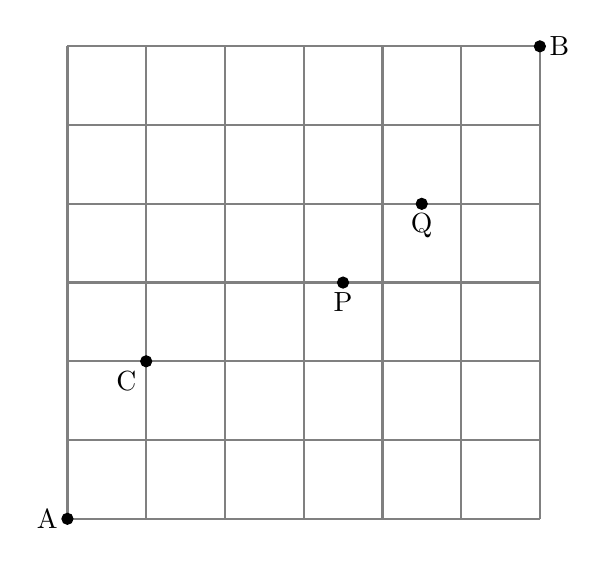
\begin{tikzpicture}
        \draw[help lines,thick](0,0)grid(6,6);
        \coordinate(A)at(0,0);
        \coordinate(C)at(1,2);
        \coordinate(P)at(3.5,3);
        \coordinate(Q)at(4.5,4);
        \coordinate(B)at(6,6);
        \node[left] at(A){A};
        \node[below left]at(C){C};
        \node[below]at(P){P};
        \node[below]at(Q){Q};
        \node[right]at(B){B};
        \filldraw[fill=black,draw=black](A)circle(2pt);
        \filldraw[fill=black,draw=black](B)circle(2pt);
        \filldraw[fill=black,draw=black](C)circle(2pt);
        \filldraw[fill=black,draw=black](P)circle(2pt);
        \filldraw[fill=black,draw=black](Q)circle(2pt);
    \end{tikzpicture}
\end{center}
\kakkoichi 地点Cを通る.\\
\kakkoni 地点Pを通る.\\
\kakkosan 地点P及び地点Qを通らない.\\
\hspace{10cm}(東北大)\\\\
\ba{6$\bullet$2}
\begin{align*}
    a+b+c+d=10\cdots\cdots\maruichi を満たす整数a,b,c,dについて,
\end{align*}
\kakkoichi 正の整数の組$(a,b,c,d)$は何通りあるか.\\
\kakkoni $0$以上の整数の組$(a,b,c,d)$は何通りあるか.\\
\kakkosan $a\geq0,b\geq1,c\geq2,d\geq3$を満たす整数の組$(a,b,c,d)$は何通りあるか.
\newpage
\begin{center}
    \ans{6章の問題演習}
\end{center}
\noindent\reibanichi \\
\kakkoichi $0<a<b<c<11$を満たす整数の組$(a,b,c)$は何通りあるか.\\
\kakkoni $0\leq a\leq b \leq c\leq11$を満たす整数の組$(a,b,c)$は何通りあるか.\\\\
\reibanni 次の条件を満たす正の整数全体の集合を$S$とおく.
\begin{align*}
    「各桁の数字は互いに異なり,どの二つの桁の数字の和も9にならない.」
\end{align*}
ただし,$S$の要素は$10$進法で表す.また,1桁の正の整数は$S$に含まれるとする.このとき次の問いに答えよ.\\
\kakkoichi $S$の要素でちょうど4桁のものは何個あるか.\\
\kakkoni 小さい方から数えて$2000$番目の$S$の要素を求めよ.\\
\hspace{10cm}(東京大)
\newpage
\section{確率の一番大切なこと}
\noindent\begin{itembox}
    [l]{\enpitu 根本事象と標本空間}
    \doichi ある試行において,起こり得る結果を「事象」という.\\
    \doni それ以上分割する意味がない.と判断した事象を根本事象(素事象)という.\\
    (ex.)「3本当たりは入っている9本のくじ引きで,1回目で当たりを引く確率.」\\
    $\xrightarrow{分割}「晴れの日に当たりを引く」「来週の火曜日に当たりを引く」「今日の放課後に当たりを引く」$\\
    こんなに事象を分けても意味ないので,問題文の状況が今回の根本事象です.\\
    \dosan 素事象全体の集合を「標本空間」という.\\
    \doshi 何を素事象にするかはあなた次第.標本空間もその時々で変わる.
\end{itembox}\\
\begin{itembox}
    [l]{\enpitu 公理的確率論(確率のちゃんとした定義)}
    $a_i(i=1,2,3,\cdots,n)$を素事象とする標本空間$S=\{a_1,a_2,a_3,\cdots,a_n\}$
    に対し,確率を次のように定義する.\\
    \doichi　 素事象$a_1,a_2,a_3,\cdots,a_n$の起こりやすさの比が
    \begin{center}
        $p(a_1):p(a_2):p(a_3):\cdots:p(a_n)$
    \end{center}
    と定まっており,
    \begin{center}
        $p(a_1)+p(a_2)+p(a_3)+\cdots+p(a_n)=1　(\temarkua これを「正規化」という)$
    \end{center}
    をみたすようにおいたとき
    \begin{center}
        $P(a_k)=\dfrac{p(a_k)}{p(a_1)+p(a_2)+p(a_3)+\cdots+p(a_n)}$
    \end{center}
    を「素事象$a_k$の確率」と定義する.\\
    \doni　 $S$の部分集合$A$に対し,「事象$A$の確率」を
    \begin{center}
        $A$に属する素事象の確率の総和
    \end{center}
    で定義する.
\end{itembox}
\newpage
\begin{itembox}
    [l]{\enpitu ラプラスの確率}
    $a_k（k=1,2,\cdots,N）$を素事象とする$N$個の素事象からなる標本空間
    \begin{align*}
        S=\B{a_1,a_2,a_3,\cdots,a_N}
    \end{align*}
    に対し,素事象$a_1,a_2,a_3,\cdots,a_N$の起こりやすさが全て同じであるという根拠があるとき,これらの素事象は
    \begin{align*}
    「同様に確からしい」
    \end{align*}
    という.このとき,各素事象の確率はすべて$\dfrac{1}{N}$なので,事象$A$に属する素事象の個数が$K$であれば,
    \begin{align*}
        P\p{A}=\dfrac{K}{N}
    \end{align*}
    となる.すなわち,
    \begin{align*}
        確率すべて同様に確からしい素事象の個数の比
    \end{align*}
    と計算することができる.
\end{itembox}\\
\begin{itembox}
    [l]{\enpitu 包除原理}
    一般に,集合$A$と集合$B$について,$A\neq B$かつ$A=B=\emptyset$であるとき,以下が成立する.
    \begin{align*}
        &\bullet n\p{A\cup B}=n\p{A}+n\p{B}-n\p{A\cap B}\\
        &\bullet n\p{A\cap B}=n\p{A}+n\p{B}-n\p{A\cup B}
    \end{align*}
\end{itembox}\\
\begin{itembox}
    [l]{\enpitu 排反と包除原理}
    一般に,
    \begin{align*}
        P\p{A\cup B}=n\p{A}+n\p{B}-n\p{A\cap B}
    \end{align*}
    が成立し,特に,$A\cap B=\emptyset（空集合）$のとき,
    \begin{align*}
        AとBは排反である
    \end{align*}
    という.このとき,
    \begin{align*}
        P\p{A\cup B}=P\p{A}+P\p{B}
    \end{align*}
    である.
\end{itembox}\\
\begin{itembox}
    [l]{\enpitu 余事象の定理}
    標本空間$S$に対し,
    \begin{align*}
        P\p{S}=1
    \end{align*}
    であり,$A\cup \overline{A}=S$,さらに$Aと\overline{A}$は排反であるので,包除原理より,
    \begin{align*}
        P\p{A}+P\p{\overline{A}}=1\doti P\p{\overline{A}}=1-P\p{A}
    \end{align*}
    である.\\
    これを素事象の定理という.
\end{itembox}
\newpage
\noindent\ba{7$\bullet$1}\\
$1,2,3,4,5,6$の目の出やすさが$1:1:1:2:2:3$であるような変なサイコロがある.このサイコロを一回投げたとき,
次のように事象$A$と$B$を定める.
\begin{align*}
    &A：奇数の目がでる\\
    &B：5以上の目がでる
\end{align*}
このとき,次の確率を全て求めよ.\\
\begin{center}
    $P\p{A},P\p{B},P\p{\overline{B}},P\p{A\cup B},P\p{A\cap B},P\p{\overline{A}\cup \overline{B}}$
\end{center}
\ba{7$\bullet$2}\\
8個中3個が当たりのくじ引きを一人一本ずつ順番に引いていく.\\
\kakkoichi 3人目があたる確率を求めよ.\\
\kakkoni 3人目か6人目の少なくとも一方が当たる確率を求めよ.\\\\
\ba{7$\bullet$3}\\
A,A,B,Bの4文字を円形に並べたとき,AとBが交互に並ぶ確率を求めよ.
\newpage
\begin{center}
    \ans{7章の問題演習}
\end{center}
\reibanichi\\
\kakkoichi 10円玉2枚を同時に投げるとき,表と裏が1枚ずつ出る確率を求めよ.\\
\kakkoni 3人でじゃんけんを1回する.「あいこ」（勝者と敗者が0）になる確率を求めよ.\\
\kakkosan $n(\geq2)$人でじゃんけんを1回する.「あいこ」になる確率を求めよ.\\
\kakkoshi 赤玉3個,白玉3個を円形に並べるとき,同じ色の玉が隣り合わない確率を求めよ.\\\\
\reibanni　7本中3本が当たりのくじを7人が順に引く.引いたくじは戻さない.\\
\kakkoichi 3人目が当たる確率を求めよ.\\
\kakkoni 6人目が当たる確率を求めよ.\\
\kakkosan 3人目と6人目がともに当たる確率を求めよ.\\
\kakkoshi 当たった人が全員奇数番目に引いた人である確率を求めよ.
\newpage
\section{条件付き確率・独立反復試行}
\begin{itembox}
    [l]{\enpitu 条件付き確率}
    事象Aが起きた（起こる）という前提の下で,事象Bが起こる（起こっていた）確率のことを
    \begin{center}
        「Aの下でのBの条件付き確率」
    \end{center}
    といい,
    \begin{center}
        $P_A(B)$
    \end{center}
    と表す.
\end{itembox}\\
\begin{itembox}
    [l]{\enpitu 積の法則}
    事象Aが空集合（$\emptyset$）でないとき,
    \begin{center}
        $P_A(B)=\dfrac{P\p{A\cap B}}{P\p{A}}\doti P\p{A\cap B}=P\p{A}P_A(B)$
    \end{center}
\end{itembox}\\
\begin{itembox}
    [l]{\enpitu 反復試行の確率}
    確率$p$で成功するような試行を独立に$n$回反復しておこなったとき,$n$回中$k$回成功する確率は,
    \begin{center}
        $\comb{n}{k}p^k\p{1-p}^{n-k}$
    \end{center}
    である.
\end{itembox}
\newpage
\noindent\ba{8$\bullet$1}\\
　7本中3本が当たりのくじを7人が順に引く.引いたくじは戻さない.\\
\kakkoichi 2人目が当たる確率を求めよ.\\
\kakkoni 2人目と6人目がふたりとも当たる確率を求めよ.\\
\kakkosan 2人目が当たったとき,6人目が当たる確率を求めよ.\\
\kakkoshi 6人目が当たったとき,2人目が当たっていた確率を求めよ.\\\\
\ba{8$\bullet$2}\\
袋の中に,両面とも赤のカードが2枚,両面とも青,両面とも黄,片面が赤で片面が青,片面が青で片面が黄のカードがそれぞれ1枚ずつ
計6枚のカードが入っている.そのうち1枚を無作為に選んで取り出し机の上に置き,それを袋には戻さずにもう1枚のカードを取り出して
机の上に置くことにする.\\
\kakkoichi 1枚目の表が赤である確率を求めよ.\\
\kakkoni 1枚目が両面とも赤である確率を求めよ.\\
\kakkosan 1枚目の表が赤であることが分かったとき,そのカードの裏も赤である確率を求めよ.\\
\kakkoshi 1枚目のカードの表が赤であると分かっているとき,2枚目のカードの表が青である確率を求めよ.\\
\kakkogo 1枚目のカードの表が赤で,2枚目のカードの表が青であることが分かったとき,1枚目のカードの裏が赤である確率を
求めよ.\\\\
\ba{8$\bullet$3}\\
サイコロを5回投げたとき,1の目がちょうど3回出る確率を\ans{まず,公式を使わずに}求めよ.\\
次に公式を使って求めよ.\\\\
\ba{8$\bullet$4}\\
AチームとBチームがサッカーの試合を7試合行う.どの試合でも,Aチームが勝つ確率は$\dfrac{1}{2}$,Bチームが勝つ確率は$\dfrac{1}{6}$,
引き分けとなる確率は$\dfrac{1}{3}$であるとして,Aチームの試合結果が3章2敗2引き分けとなる確率を求めよ.
\newpage
\begin{center}
    \ans{8章の問題演習}
\end{center}
\noindent\reibanichi 袋の中に赤玉4個と白玉6個が入っている.Aが玉を2個取り出し,取り出した玉の色を確認して,もし2個とも赤玉なら赤玉1個を,
それ以外の場合は白玉1個を袋に戻し,次にBがその袋から玉を2個取り出す.次の問いに答えよ.\\
\kakkoichi Aが白玉2個を取り出し,かつBが赤玉2個を取り出す確率を求めよ.\\
\kakkoni Bが赤玉2個を取り出す確率を求めよ.\\
\kakkosan Bが取り出した玉が赤玉2個であったとき,Aが取り出した玉が白玉2個である条件付き確率を求めよ.\\
\hspace{10cm}(琉球大)\\\\
\reibanni 座標平面上で$x$座標と$y$座標がいずれも整数である点を格子点という.格子点上を次の規則にしたがって動く点Pを考える.
\begin{align*}
    (a)&最初に,点\mathrm{P}は原点\mathrm{O}にある.\\
    (b)&ある時刻で点\mathrm{P}が格子点(m,n)にあるとき,その1秒後の点\mathrm{P}の位置は,隣接する格子点\\
    &(m+1,n),(m,n+1),(m-1,n)(m,n-1)
    のいずれかであり,また,これらの点に移動する確率は,\\
    &それぞれ\frac{1}{4}である.
\end{align*}
\kakkoichi 点Pが,最初から6秒後に直線$y=x$上にある確率を求めよ.\\
\kakkoni 点Pが,最初から6秒後に原点Oにある確率を求めよ.\\
\hspace{10cm}(東京大)\\\\
\reibansan $n$を2以上の自然数とする.さいころを$n$回振り,出た目の最大値$M$と最小値$L$の差$M-L$を$X$とする.\\
\kakkoichi $X=1$である確率を求めよ.\\
\kakkoni $X=5$である確率を求めよ.\\
\hspace{10cm}(京都大)
\newpage
{\LARGE\ans{論理に関するチェックテスト}}\\
これから,数学において最も大事であると言ってよい「論理」を勉強していきます.その前にどれだけ皆さんが
数学の言語を読むことができていないのか明らかにしていきましょう.\\
深く考えずに1問10秒を目安に「A:正しい」「B:誤り」で答えてみてください.\\
\kakkoichi 「3は偶数である」という主張は命題である.\\
\kakkoni 「$2n$は偶数である」という主張は命題である.\\
\kakkosan 「2は偶数」または「3は偶数」\\
\kakkoshi 「2が奇数」ならば「$3+2=1$」\\
\kakkogo 実数$x$を上手く選ぶと$x^2+x+1=0$が成立する.\\
\kakkoroku $x^{2345}+x^{1234}+x-1=0$となる実数$x$が存在する.\\
\kakkoshichi $x^2\geq4$を満たす任意の$x$に対し$x\geq2$が成立する.\\
\kakkohachi $x^2\geq4$を満たすある$x$に対し$x\geq100$が成立する.\\
\kakkokyu 適当な$x$をとれば任意の$y$に対して$x>y$\\
\kakkojyu 任意の$y$に対して適当な$x$をとれば$x>y$\\
\kakkojyuichi 「すべての$x$に対してある$y$が存在して任意の$k$に対して$x+y^2=K$となる」は命題である.\\
\kakkojyuni ある鈍角$\theta$に対し,$\dfrac{1}{1234}\cos\theta+\dfrac{100}{99}\sin\theta=1$\\
\kakkojyusan 「$0\leq x\leq1$ 」ならば「$x^2\leq2$」\\
\kakkojyushi 「$1\leq x\leq0$」ならば「$x^2\leq2$」\\
\kakkojyugo $x^2=1$であるためには$x=1$であることが必要.\\
\kakkojyuroku 「$A<B$」が分かっている.「$A<C$」を示すためには「$B<C$」を示す必要がある.\\
\kakkojyushichi 任意の$x$に対し$ax^2+bx+c<0$が成立するためには$a<0$が必要である.\\
\kakkojyuhachi $a=b^c$ならば$c=\log_b a$である.\\
\kakkojyukyu 「$\alpha=\beta$」ならば「$\tan\alpha=\tan\beta$」\\
\kakkonijyu 「$\tan\alpha=\tan\beta$」ならば「$\alpha=\beta$」\\
(21)関数$f(x)$がすべての$x$に対して$f(x)\geq1$を満たすならば,$f(x)$の最小値は1である.\\
(22)関数$f(x)$がすべての実数$x$に対して$f(x)>0$を満たすならば,$f(x)$の最小値は正である.\\
(23)$x\neq0$ならば$(x,y)\neq(0,0)$である.\\
(24)$x\neq0$ならば$x\neq0$かつ$y\neq0$である.\\
(25)$a>b$ならば$a\geq b$である.\\
(26)$a>b$ならば$a^2>b^2$である.\\
(27)$a\geq\sqrt{b}$ならば$a^2\geq b$である.\\
(28)$a\leq\sqrt{b}$ならば$a^2\leq b$である.\\
(29)$ab=c$ならば$a=\frac{c}{b}$である.\\
(30)$a=\dfrac{c}{b}$ならば$ab=c$である.\\
(31)3点A,B,Pが同一直線上にあるなら,$\Vec{AP}=k\Vec{AB}$の形で表せる.\\
(32)「単位円周上の点PはP$\p{\cos\theta,\sin\theta}$の形で表せる」は$\theta$の条件である.\\
(33)$(3,2)$を通る$xy$平面上の直線は$y=m(x-3)+2$の形で表せる.\\
(34)整数$m$を4で割った余りが3のとき,$m=4k+3（kは整数）$である.\\
(35)二つの平面ベクトル$\vec{a},\vec{b}$が一次独立のとき,ある実数$p,q$が存在して,平面上のすべて
の点Pに対し$\Vec{OP}=p\vec{a}+q\vec{b}$である.\\
(36)直線$y=x+1$上の任意の点$(x,y)$について,\\すべての実数$t$に対して,$\tvec<0,1>[x,y]=\tvec<0,1>[0,1]+t\tvec<0,1>[1,1]$である.\\
\theme{解答欄}
\begin{center}
    \begin{tabular}{|c|c|c|c|c|c|c|c|c|c|c|c|}
        \hline
        (1)&(2)&(3)&(4)&(5)&(6)&(7)&(8)&(9)&(10)&(11)&(12)\\
        \hline
        {}&{}&{}&{}&{}&{}&{}&{}&{}&{}&{}&{}\\
        \hline
        \hline
        (13)&(14)&(15)&(16)&(17)&(18)&(19)&(20)&(21)&(22)&(23)&(24)\\
        \hline
        {}&{}&{}&{}&{}&{}&{}&{}&{}&{}&{}&{}\\
        \hline
        \hline
        (25)&(26)&(27)&(28)&(29)&(30)&(31)&(32)&(33)&(34)&(35)&(36)\\
        \hline
        {}&{}&{}&{}&{}&{}&{}&{}&{}&{}&{}&{}\\
        \hline
    \end{tabular}
\end{center}
\newpage
\section{論理1(命題と条件)}
\begin{itembox}
    [l]{\enpitu 主張・命題・条件}
    \kakkoichi 「$A$は$B$である」という形の文を\ans{主張}という.\\
    \kakkoni 正しい(真)か正しくない(偽)かが判定できる主張を\ans{命題}という.\\
    \kakkosan 文字を含んでおり,その文字に具体的な数値を代入することで真偽が定まり命題となるような主張を,\ans{その文字の条件}という.
\end{itembox}\\
ex)\\
$\bullet$「$1+3$」は主張ではない.\\
$\bullet$「$1+3>5$」は偽の命題.\\
$\bullet$「$a+b>5$」は$a,b$の条件.\\
$\bullet$「$x^2-2x+1=0$」は$x$の条件.\\
$\bullet$「$ax^2-2x+1=0$」は$a,x$の条件.\\
$\bullet$「$x$の二次方程式$x^2-2x+1=0$は少なくとも一つ実数解を持つ」は真の命題.\\
$\bullet$「$x$の二次方程式$x^2-2kx+1=0$は少なくとも一つ実数解を持つ」は$k$の条件.\\
$\bullet$「$\lim_{n\to\infty}a_n$が収束する」は数列$\B{a_n}$の条件.\\\\
\begin{itembox}
    [l]{\enpitu 論理記号の定義1(主張)}
    以下,$p.q$を命題とする.
    \begin{align*}
        &「pが成り立っていない」という主張を\neg p（\leftrightarrow\overline{p}）と表す.\\
        &「pとq両方とも成り立っている」という主張をp\wedge qと表す.\\
        &「pならばq」という主張をp\narabaa qと表す.
    \end{align*}
真の命題を$\bigcirc$,偽の命題を$\times$で表すと,それぞれの定義は下表のようになる.\\\\
\hspace{2cm}
\begin{tabular}{|c||c|}
    \hline
    $p$&$\neg p$\\
    \hline
    $\bigcirc$&$\times$\\
    \hline
    $\times$&$\bigcirc$\\
    \hline
\end{tabular}
\hspace{3cm}
\begin{tabular}{|c|c||c|c|c|}
    \hline
    $p$&$q$&$p\wedge q$&$p\vee q$&$p\narabaa q$\\
    \hline
    $\bigcirc$&$\bigcirc$&$\bigcirc$&$\bigcirc$&$\bigcirc$\\
    \hline
    $\bigcirc$&$\times$&$\times$&$\bigcirc$&$\times$\\
    \hline
    $\times$&$\bigcirc$&$\times$&$\bigcirc$&$\bigcirc$\\
    \hline
    $\times$&$\times$&$\times$&$\times$&$\bigcirc$\\
    \hline
\end{tabular}\\
上表を真理値表という.
\end{itembox}\\
\begin{itembox}
    [l]{\enpitu 命題の同値性}
    $P,Q,R$を命題とする.その真偽に関わらず,次の関係が成り立つ.
    \begin{align*}
        &\kakkoichi \neg\p{\neg P}\doti P（二重否定）\\
        &\kakkoni\begin{cases}
            \neg\p{P\wedge Q}\doti \p{\neg P}\vee\p{\neg Q}\\
            \neg\p{P\vee Q}\doti \p{\neg P}\wedge\p{\neg Q}
        \end{cases}（大人向けド・モルガンの法則）\\
        &\kakkosan\p{P\narabaa Q}\doti \p{\neg Q\narabaa \neg P}（対偶）\\
        &\kakkoshi\begin{cases}
            P\wedge\p{Q\vee R}\doti \p{P\wedge Q}\vee\p{P\wedge R}\\
            P\vee\p{Q\wedge R}\doti \p{P\vee Q}\wedge\p{P\vee R}
        \end{cases}（主張の分配法則）
    \end{align*}
\end{itembox}
\chud：命題を繋ぐ同値記号は実は$\doti$では正しくない.正しくは$「\leftrightarrow」もしくは「\godo」$で繋ぐのが正しい.\\
ただし,誤解の恐れがない場合や以後の問題に支障をきたさない場合,それらを区別せず$\doti$ の記号を用いる.
\newpage
\begin{itembox}
    [l]{\enpitu 真理集合}
    条件$P$を真にするような集合の全体を,条件$P$の真理集合という.\\
    ex)\\
    $\bullet$\hspace{2mm}$x$の条件$P(x)$の真理集合は,$\B{x|P(x)}$である.\\
    $\bullet$\hspace{2mm}$a,b$の条件$P(a,b)$の真理集合は,$\B{\tvec[a,b]|P(a,b)}$である.\\\\
    一文字の条件の真理集合は数直線上に,二文字の条件の真理集合は平面上に図示して表現することがよくある.
\end{itembox}\\
\begin{itembox}
    [l]{\enpitu 論理記号の定義2(量化記号)}
    $P(x)$を$x$の条件とする.
    \begin{align*}
        &\kakkoichi 「すべてのxに対してP(x)が成立する.」という主張を 「\forall x,P(x)」と書く.\\
        &\kakkoni 「少なくとも一つのxに対してP(x)が成立する.」という主張を「\exists x,P(x)」と書く.
    \end{align*}
\end{itembox}\\
\chud\\
量化記号$\forall と\exists$には様々な別表現がある.\\
\begin{itembox}
[l]{\enpitu 量化記号と主張}
$x$の取とり得る値が$x_1,x_2,\cdots,x_n$のとき,
\begin{align*}
    &\kakkoichi \forall x,P(x)\doti P(x_1)\wedge P(x_2)\wedge P(x_3)\wedge\cdots\wedge P(x_n)\\
    &\kakkoni \exists x,P(x)\doti P(x_1)\vee P(x_2)\vee P(x_3)\vee\cdots\vee P(x_n)
\end{align*}    
\end{itembox}
\newpage
\noindent\ba{9$\bullet$1}\\
$P,Q$を命題とするとき,その真偽に関わらず,命題の同値関係
\begin{center}
    $\p{P\narabaa Q}\doti \p{\neg P\vee Q}$
\end{center}
が成立することを,下記の真理値表を用いて証明せよ.
\begin{center}
    \begin{tabular}{|c|c||c|c|c|}
        \hline
        $P$&$Q$&$\neg P$&$P\narabaa Q$&$\neg P\vee Q$\\
        \hline
        $\bigcirc$&$\bigcirc$&{}&{}&{}\\
        \hline
        $\bigcirc$&$\times$&{}&{}&{}\\
        \hline
        $\times$&$\bigcirc$&{}&{}&{}\\
        \hline
        $\times$&$\times$&{}&{}&{}\\
        \hline
        \end{tabular}
\end{center}
\ba{9$\bullet$2}\\
次の各文を「A:真の命題」,「B:偽の命題」,「C:条件」,「D:いずれでもない」に分類せよ.また「C:条件」の場合はその真理集合を求めよ.ただし,文字はすべて実数の
範囲で考えよ.\\
\kakkoichi 「$\neg(1+1=3)$」\\
\kakkoni 「$1+1=3\vee1+2=3$」\\
\kakkosan 「$1+1=3\narabaa 1+2=3$」\\
\kakkoshi 「$x^2+4x-1$」\\
\kakkogo 「$x^2+4x-1=0$」\\
\kakkoroku「$x^2+4x-1=0$を満たす実数$x$は二つある.」\\
\kakkoshichi「すべての実数$x$に対して,$x^2+4x+5>0$である.」\\
\kakkohachi「ある実数$x$に対して,$x^2+4x+5<0$である.」\\
\kakkokyu「$\forall x,x^2>-1$」\\
\kakkojyu「$\forall x,x^2>1$」\\
\kakkojyuichi「$\exists x,x^2>-1$」\\
\kakkojyuni「$\exists x,x^2<1$」\\
\kakkojyusan「$\forall x,x^2>k$」\\
\kakkojyushi「$\exists x,x^2<k$」
\newpage
\begin{center}
    \ans{9章の問題演習}
\end{center}
\noindent\reibanichi $P,Q$を命題とする.3つの命題
\begin{align*}
    \tokeiichi P\narabaa Q,\tokeini Q\narabaa P,\tokeisan \neg P\narabaa \neg Q
\end{align*}
に対して,\\
\kakkoichi \tokeiichi と\tokeini の真偽は必ずしも一致しないことを示せ.\\
\kakkoni \tokeiichi と\tokeisan の真偽は必ずしも一致しないことを示せ.\\
\kakkosan \tokeini と\tokeisan の真偽は必ず一致することを示せ.\\\\
\reibanni $P,Q,R$を命題とするとき,その真偽に関わらず,次の命題の同値関係が成立することを示せ.
\begin{center}
    $P\wedge\p{Q\vee R}\doti\p{P\wedge Q}\vee \p{P\wedge R}$
\end{center}
\newpage
\section{領域の図示}
\begin{itembox}
    [l]{\enpitu 4つの領域}
    2変数関数$f(x,y)$を一つ与えたとき,$xy$平面は次の4つの領域に重複なく分割することができる.
    \begin{align*}
        &A=\B{(x,y)\left|\right.f(x,y)>0}（f(x,y)の正領域という）\\
        &B=\B{(x,y)\left|\right.f(x,y)=0}（f(x,y)の零領域という）\\
        &C=\B{(x,y)\left|\right.f(x,y)<0}（f(x,y)の負領域という）\\
        &D=\B{(x,y)\left|\right.f(x,y)が定義できない}
    \end{align*}
\end{itembox}\\
\begin{itembox}
    [l]{\enpitu 種々の移動}
    $x,y$の条件$F(x,y)$の真理集合を$P$としたとき,
    \begin{align*}
        &F(x-p,y-q)の真理集合は,Pを\tvec<0,1>[p,q] 平行移動した図形\\
        &F(-x,y)の真理集合は,Pをy軸に関して鏡映移動した図形\\
        &F(x,-y)の真理集合は,Pをx軸に関して鏡映移動した図形\\
        &F(y,x)の真理集合は,Pをy=xに関して鏡映移動した図形i.e.逆関数\\
        &F\p{\frac{x}{k},\frac{y}{k}}の真理集合は,Pを原点中心にk倍に相似拡大した図形\\
        &F\p{\frac{x}{p},\frac{y}{q}}の真理集合は,Pをx方向にp倍,y方向にq倍に偏倍拡大した図形
    \end{align*}
\end{itembox}\\
\begin{itembox}
    [l]{\enpitu 対称性}
    $x,yの条件F(x,y)$の真理集合$P$としたとき,
    \begin{align*}
        &「F(-x,y)\narabaa F(x,y)」\narabaa 「Pはy軸対称」\\
        &「F(x,-y)\narabaa F(x,y)」\narabaa 「Pはx軸対称」\\
        &「F(-x,-y)\narabaa F(x,y)」\narabaa 「Pは原点対称」\\
        &「F(y,x)\narabaa F(x,y)」\narabaa 「Pは直線y=xについて対称」
    \end{align*}
\end{itembox}
\newpage
\noindent\ba{10$\bullet$1}\\
$f(x,y)=\sqrt{x}-y$に対し,$xy$平面を次の4つの領域に塗り分けよ.
\begin{align*}
    &A=\B{(x,y)\left|\right.f(x,y)>0}\\
        &B=\B{(x,y)\left|\right.f(x,y)=0}\\
        &C=\B{(x,y)\left|\right.f(x,y)<0}\\
        &D=\B{(x,y)\left|\right.f(x,y)が定義できない}
\end{align*}
\ba{10$\bullet$2}\\
次の不等式の表す領域を図示せよ.\\
\kakkoichi$xy\leq1$\\
\kakkoni$y\leq\frac{1}{x}$\\
\kakkosan$(x+y)(x-y-2)(x^2+y^2-1)\leq0$\\
\kakkoshi$(y-\tan x)(x+y)(y-1)<0\wedge-\frac{\pi}{2}<x<\frac{\pi}{2}$\\
\kakkogo$(\sin2y\geq\sin x)\wedge\p{0\leq x\leq2\pi}\wedge\p{0\leq y\leq2\pi}$\\\\
\ba{10$\bullet$3}\\
次の不等式の表す領域を図示せよ.\\
\kakkoichi $y\leq x^2-2|x|-3$\\
\kakkoni$|y|\leq\left|x^2-2x-3\right|$\\
\kakkosan$1\leq\left|\left|x\right|-2\right|+\left|\left|y\right|-2\right|\leq3$
\newpage
\begin{center}
    \ans{10章の問題演習}
\end{center}
\noindent\reibanichi 次の不等式の表す領域を図示せよ.\\
\kakkoichi$xy\geq1$\\
\kakkoni$(2-xy)(x^2+y^2-5)\leq0$\\
\kakkosan$(x-1)(x+y)(x-y+2)<0$\\
\kakkoshi$x(x^2+y-2)(x-y)^2\geq0$\\
\kakkogo$(\cos2y<\cos x)\wedge\p{0<x<2\pi}\wedge\p{0<y<2\pi}$\\
\kakkoroku$2\leq\left|\left|x\right|-2\right|+\left|\left|y\right|-1\right|\leq3$
\newpage
\noindent\chud 追加の解説があります.\\
\begin{itembox}
    [l]{\enpitu かわりばんこの法則}
    一般に,二次元平面上では零領域を境に正領域と負領域が交互に現れる.
\end{itembox}
この法則の主張を具体的にしましょう.\\
ex)$y\geq x^2$を図示せよ.\\
\kai $f(x,y)=y-x^2$とおくと,図示するべき領域は,
\begin{align*}
    f(x,y)\geq0\cdots\cdots\maruichi\doti f(x,y)の正領域
\end{align*}
である.例えば,$\maruichi$を満たすような$(x,y)$として,$\ans{(x,y)=(0,2)}$がとれる.\\
これをプロットすると,下図のようになる.
\begin{center}
    \begin{tikzpicture}[scale=0.8]
        \draw[->,>=Latex](-4,0)--(4,0)node[right]{$x$};
        \draw[->,>=Latex](0,-1)--(0,6)node[above]{$y$};
        \filldraw[draw=black,fill=black](0,2)circle(2pt);
        \node[below left]at(0,0){O};
        \begin{clip}
        (-4,-1)rectangle(4,6);
        \draw[thin,smooth]plot(\x,{pow(\x,2)});
        \node[above right]at(0,2){$\ans{(0,2)}$};
        \end{clip}
        \node[right]at(2.5,5){$y=x^2$};
    \end{tikzpicture}
\end{center}
よって,求める領域は,$y=x^2$の内部（正領域）であり,下図の網目部で境界を含む.
\begin{center}
    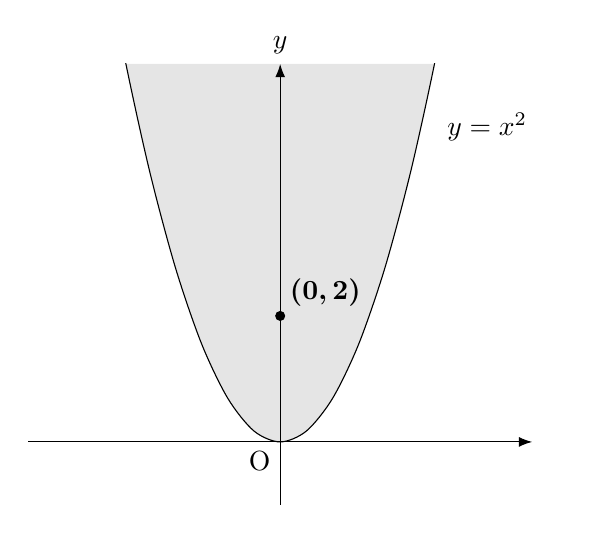
\begin{tikzpicture}[scale=0.8]
        \begin{clip}
        (-4,-1)rectangle(4,6.5);
        \fill[gray!20!white]plot[domain=-2.45:2.45](\x,{pow(\x,2)});
        \end{clip}
        \draw[->,>=Latex](-4,0)--(4,0)node[right]{$x$};
        \draw[->,>=Latex](0,-1)--(0,6)node[above]{$y$};
        \filldraw[draw=black,fill=black](0,2)circle(2pt);
        \node[below left]at(0,0){O};
        \begin{clip}
        (-4,-1)rectangle(4,6);
        \draw[thin,smooth]plot(\x,{pow(\x,2)});
        \node[above right]at(0,2){$\ans{(0,2)}$};
        \end{clip}
        \node[right]at(2.5,5){$y=x^2$};
    \end{tikzpicture}
\end{center}
\newpage
\section{全称と存在}
\begin{itembox}
    [l]{\enpitu 束縛変数と従属変数}
    $\bullet$他の文字に変えても主張の意味が変わらない文字のことを\ans{束縛変数}という.\\
    $\bullet$そうでない文字のことを\ans{自由変数}という.
\end{itembox}\\
\begin{itembox}
    [l]{\enpitu 群}
    ある集合$G$に対して,次の性質を満たすとき,$\ans{Gは群である}という.$
    \begin{align*}
        &a,b,c\in Gに対して,二項演算*が定義されているとする.\\
        &\kakkoichi a*(b*c)=(a*b)*c（結合法則が成立する）\\
        &\kakkoni \exists e\in G　s.t　\forall a\in G,a*e=e*a=a（単位元の存在）\\
        &\kakkosan \forall a\in G,\exists a^{-1},a*a^{-1}=a^{-1}*a=e（逆元の存在）
    \end{align*}
\end{itembox}\\
\begin{itembox}
    [l]{\enpitu アーベル群}
    群の\kakkoichi$\sim$\kakkosan の性質に加えて次の性質が成り立つとき,\ans{$G$はアーベル群である}という.
    \begin{align*}
        a*b=b*a（交換法則が成立する.）
    \end{align*}
    つまり,$G$に可換性を付与したものである.
\end{itembox}\\
\begin{itembox}
    [l]{\enpitu 環（ring）}
    ある集合$R$に対して,群の性質に加えて,次の性質を満たすとき,$\ans{Rは環である}$という.
    \begin{align*}
        &a,b,c\in Rに対して,以下が成立する.\\
        &・a(b+c)=ab+ac（左分配法則）\\
        &・(a+b)c=ac+bc（右分配法則）
    \end{align*}
    さらに,可換性があるものを$\ans{Rは可換環である}という.$
\end{itembox}\\
\begin{itembox}
    [l]{\enpitu 体}
    ある集合$K$に対して,可換環であって,さらに割り算ができる集合$K$を$\ans{Kは体である}$という.
\end{itembox}\\
\begin{itembox}
    [l]{\enpitu 数の集合の略記}
    \begin{align*}
        &\bullet 自然数全体の集合を\mathbb{N}で表す.\\
        &\bullet 整数全体の集合を\mathbb{Z}で表す.\\
        &\bullet 有理数全体の集合を\mathbb{Q}で表す.\\
        &\bullet 実数全体の集合を\mathbb{R}で表す.\\
        &\bullet 複素数全体の集合を\mathbb{C}で表す.\\
        &\bullet 四元数全体の集合を\mathbb{H}で表す.\\
        &\bullet 八元数全体の集合を\mathbb{O}で表す.
    \end{align*}
\end{itembox}\\
（演習）\\
次の日本語の文を論理記号を用いて書き直せ.\\
\kakkoichi $m$は0以上の整数である.\\
\kakkoni $f(x)=0$を満たすような実数$x$が少なくとも一つ存在する.\\
\kakkosan どんな実数$x$に対しても$x^2$は必ず0以上になる.\\
\kakkoshi 自然数$n$に対し定義された数列$\B{a_n}$の各項は全て整数になる.\\\\
\begin{itembox}
    [l]{\enpitu $\forall$と$\exists$の混合文}
    $\ans{\forall と\exists の順序が変わると,全く違う主張になることに注意せよ.}$
    \begin{align*}
        &ex)\\
        &\bullet \forall x,\exists y,P(x,y)と\exists y,\forall x,P(x,y)では全く意味が異なる.\\
        &\bullet \forall x,\forall y,P(x,y)と\forall y,\forall y,P(x,y)は同じ意味である.\\
        &まとめて,\forall(x,y),P(x,y)と書いたり,
        \forall\tvec<0,1>[x,y],P(x,y)と書くことが多い.\\
        &\bullet\exists x,\exists y,P(x,y)と\exists y,\exists x,P(x,y)は同じ意味である.\\
        &まとめて,\exists(x,y),P(x,y)と書いたり,
        \exists\tvec<0,1>[x,y],P(x,y)と書くことが多い.
    \end{align*}
\end{itembox}\\
\begin{itembox}
    [l]{\enpitu 0文字の条件が命題}
    次のような主張があったとする.
    \begin{align*}
        \underline{\exists a,\underline{\forall b,\underline{\exists c,(a,b,cの条件)}_{\marusan}}_{\maruni}}_{\maruichi}
    \end{align*}
    $\maruichi は,a,b,cに無関係な命題である.$\\
    $\maruni は,b,cに無関係なaの条件である.$\\
    $\marusan は,cとは無関係なa,bの条件である.$
\end{itembox}
\newpage
\noindent\ba{11$\bullet$1}\\
次の条件の真理集合を$ab$平面に図示せよ.\\
\kakkoichi$\forall x,ax+b$\\
\kakkoni$\exists x,ax+b$\\
\kakkosan$\forall x,x^2-2ax+b\geq0$\\
\kakkoshi$\exists x,ax^2-2bx-1\geq0$\\\\
\ba{11$\bullet$2}\\
次の命題の真偽を判定せよ.\\
\kakkoichi$「\forall x,\exists y,x>y」$\\
\kakkoni$「\exists y,\forall x,x>y」$\\\\
\ba{11$\bullet$3}\\
次の主張を日本語を一切使わずに数式及び数学でしようする記号のみで書き,命題の場合はその真偽を判定せよ.\\
\kakkoichi$xの2次方程式x^2+2x-1=0は有理数解をもつ.$\\
\kakkoni$\tan\theta=2を満たす鈍角\theta が存在する.$\\
\kakkosan$1<x<2を満たすすべてのxに対して,x^2-3x<0$である.\\
\kakkoshi$放物線y=x^2と直線y=x+1$は共有点を持つ.
\newpage
\begin{center}
    \ans{11章の問題演習}
\end{center}
\reibanichi 次の主張を日本語を一切使わずに数式及び数学で使用する記号のみを用いて表せ.\\
\kakkoichi $nは整数である.$\\
\kakkoni$二つのxの二次方程式x^2-x=0,x^2-2x-3=0はともに実数解をもつ.$\\
\kakkosan$二つのxの二次方程式x^2-x=0,x^2-2x-3=0は共通解をもつ.$\\
\kakkoshi$どんな正の数aに対しても,xの方程式x^2=aは実数解を持つ.$\\
\kakkogo$数列\B{a_n}は等差数列である.$\\
\kakkoroku$有理数は必ず既約分数で表せる.$\\
\kakkoshichi$xの方程式f(x)=0は少なくとも一つ実数解を持つ.$\\
\kakkohachi$xの方程式f(x)=0は異なる二つの実数解をもつ.$\\
\kakkokyu$どんな大きい数を見つけても,それより大きな数がある.$\\
\kakkojyu$関数f(x)の最大値は4である.$\\
\reibanni\\
　チェックテストの(9)$\sim$(12)を確認せよ.
\newpage
\section{必要と十分,同値変形1}
\begin{itembox}
    [l]{\enpitu 条件と条件をつなぐとは}
    $P(x),Q(x)$をそれぞれ$x$の条件とする.このとき,
    \begin{align*}
        P(x)\narabaa Q(x)　　\cdots\maruichi
    \end{align*}
    は$x$の条件であり,
    \begin{align*}
        \forall x,P(x)\narabaa Q(x)　　\cdots\maruni
    \end{align*}
    は命題である.この命題$\maruni$を先頭の$\forall x$を省略して,
    \begin{align*}
        P(x)\narabaa Q(x)　　\cdots\marusan
    \end{align*}
    と書くことが多い.ほとんどの場合,$\marusan$の意味で解釈する.\\
    つまり,
    \begin{center}
        $\ans{条件と条件をつなぐ\narabaa は先頭に\forall が省略されていると考えよ.}$
    \end{center}
\end{itembox}\\
\begin{itembox}
    [l]{\enpitu 前提条件}
    $p,q,r$を条件とする.
    \begin{align*}
        p\wedge q\narabaa p\wedge r
    \end{align*}
    という主張を,
    \begin{align*}
        pの下で,q\narabaa r
    \end{align*}
    や
    \begin{align*}
        pのとき,q\narabaa r
    \end{align*}
    などと言うことがある.この$p$を「前提条件」という.\\
    \chu これは,$\ans{(pのときq)\narabaa r}$とは全く違う主張であることに注意せよ.
\end{itembox}
\newpage
\begin{itembox}
    [l]{\enpitu 必要条件と十分条件と部分集合}
    二つの条件$p,q$の真理集合をそれぞれ,$P,Q$とする.このとき,
    \begin{center}
        $P\narabaa Q\doti P\subset Q$
    \end{center}
    である.\\
    これは,「札幌と北海道」や「東京と東久留米」と解釈すれば当たり前である.
\end{itembox}\\
まずは,必要と十分の演習です.\\
\ba{12$\bullet$1}\\
文字は全て実数で考えるものとする.このとき,以下に質問に答えよ.また,$\doti$の質問において,正しくないならば$\marubatu,\batumaru,\batubatu $のいずれなのか答えよ.\\
\kakkoichi 「$1+1=0\narabaa 1+1=1」$は正しいか.\\
\kakkoni $「x>1\narabaa x^2>1」$は正しいか.\\
\kakkosan $「x^2>1\narabaa x>1」$は正しいか.\\
\kakkoshi $「y=\sqrt{x}\doti y^2=x」$は正しいか.\\
\kakkogo $「y\geq\sqrt{x}\doti y^2\geq x」$は正しいか.\\
\kakkoroku$「y\leq\sqrt{x}\doti y^2\leq x」$は正しいか.\\
\chu \kakkoshi$\sim$\kakkoroku は次回の同値変形2で扱います.
\newpage
ここからは,「分数関数」「絶対値」の同値変形を扱います.すべての同値変形は考えれば当たり前です.自分で作れるようにしてください.\\
\begin{itembox}
    [l]{\enpitu 分数の処理}
    文字はすべて実数とする.
    \begin{align*}
        &\kakkoichi \dfrac{A}{B}=0\doti \begin{cases}
            A=0\\
            B\neq0
        \end{cases}\\\\
        &\kakkoni \dfrac{A}{B}>0\doti AB>0\\
        &\kakkosan \dfrac{A}{B}<0\doti AB<0\\
        &\kakkoshi \dfrac{A}{B}\geq0\doti\begin{cases}
            AB\geq0\\
            B\neq0
        \end{cases}\\\\
        &\kakkogo\dfrac{A}{B}\leq0\doti\begin{cases}
            AB\leq0\\
            B\neq0
        \end{cases}
    \end{align*}
\end{itembox}\\
\begin{itembox}
    [l]{\enpitu 絶対値の処理}
    文字はすべて実数とする.
    \begin{align*}
        &\kakkoichi\sqrt{A^2}=\left|A\right|\\
        &\kakkoni A\geq0のとき,\left|A\right|=A,　A\leq0のとき,\left|A\right|=-A\\\\
        &\kakkosan \left|A\right|=k\doti\begin{cases}
            k\geq0\\
            A=\pm k
        \end{cases}\\\\
        &\kakkoshi\left|A\right|<k\doti-k<A<k\\
        &\kakkogo\left|A\right|>k\doti (A>k)\vee (A<-k) 
    \end{align*}
\end{itembox}
\newpage
\noindent\ba{12$\bullet$2}\\
次の不等式を解け.
\begin{align*}
    \dfrac{4(x-1)}{x}\leq4-x
\end{align*}
 \hspace{10cm}（大阪大）\\\\
\ba{12$\bullet$3}\\
次の方程式・不等式を解け.\\
\kakkoichi $\left|x^2-2x-4\right|=x+1$\\
\kakkoni $\left|2x-1\right|+\left|x+2\right|<4$\\\\
\ba{12$\bullet$4}\\
次の条件の真理集合を同値変形で変形したのちに図示せよ.\\
\kakkoichi$x=\dfrac{2}{1+\p{\frac{y}{x}}^2}$\\
\kakkoni$\dfrac{1}{x}-\dfrac{1}{y}\geq1$\\
\kakkosan$\left|x+y\right|+\left|x-y\right|\leq1$
\newpage
\begin{center}
    \ans{12章の問題演習}
\end{center}
\reibanichi 次の空欄に当てはまるものを,下の(a)$\sim$(d)から選べ.\\
\kakkoichi 実数$x$について,$x=1$であることは,$x^2+3x-4=0$であるための\Bc{ア}.\\
\kakkoni 実数$x,y$について,$\begin{cases}
    x+y=1\\
    y=0
\end{cases}$であることは,$x=1$であるための\Bc{イ}.\\
\kakkosan 実数$x,y$について,$x^2+y^2\leq1$であることは,$|x|+|y|\leq1$であるための\Bc{ウ}.\\\\
(a)必要十分条件である\\
(b)必要条件であるが,十分条件ではない\\
(c)十分条件であるが,必要条件ではない\\
(d)必要条件でも十分条件でもない\\\\
\reibanni チェックテストの\kakkojyusan$\sim$(24) を確認せよ.\\\\
\reibansan 次の方程式・不等式を同値変形により解け.\\
\kakkoichi $\dfrac{1}{x-1}+\dfrac{2}{x-2}\leq1$\\
\kakkoni$|x-5|-|2x+1|=1$\\
\kakkosan$|2x-1|+|x-1|<3$\\\\
\reibanshi チェックテストの(29)$\sim$(30)を確認せよ.
\newpage
\section{同値変形2（無理方程式,maxとmin）}
\begin{itembox}
    [l]{\enpitu 両辺を2乗するとは}
    両辺を2乗する行為は,大抵同値性がくずれた正しくない変形になります.
    \begin{align*}
        &\bullet x=y\marubatu x^2=y^2\\
        &\bullet x>y\batubatu x^2>y^2\\
        &「xとyが同符号のとき,x=y」\marumaru x^2=y^2\\
        &「x,y\geq0のとき,x>y」\marumaru x^2>y^2
    \end{align*}
\end{itembox}\\
\begin{itembox}
    [l]{\enpitu $y=\sqrt{x}$の同値変形}
    \begin{center}
        $y=\sqrt{x}\doti\begin{cases}
            y^2=x\\
            y\geq0
        \end{cases}$
    \end{center}
    自分で導きましょう.
\end{itembox}\\
\begin{itembox}
    [l]{\enpitu $y>\sqrt{x}$の同値変形}
    \begin{center}
        $y>\sqrt{x}\doti\begin{cases}
            y^2>x\\
            x\geq0\\
            y\geq0（y>0でも良い）
        \end{cases}$
    \end{center}
    これも自分で導きましょう.
\end{itembox}\\
\begin{itembox}
    [l]{\enpitu $y<\sqrt{x}$の同値変形}
    \begin{center}
        $y<\sqrt{x}\doti\p{y^2<x}\vee\begin{cases}
            x\geq0\\
            y<0
        \end{cases}$
    \end{center}
    これも自分で導きましょう.
\end{itembox}\\
\begin{itembox}
    [l]{\enpitu $\max,\min$の同値変形}
    あまり出題されませんが,一応やります.考えれば当たり前です.
    \begin{align*}
        &\max\B{x,y}<k\doti x<k\wedge y<k\\
        &\max\B{x,y}>k\doti x>k\vee y>k\\
        &\min\B{x,y}<k\doti x<k\vee y<k\\
        &\min\B{x,y}>k\doti x>k\wedge y>k
    \end{align*}
\end{itembox}
\newpage
\noindent\ba{12$\bullet$1}\\
次の不等式を解け.
\begin{align*}
    \sqrt{2\p{x-2}\p{x^2-2}}>2-x-x^2
\end{align*}
\hspace{5cm}（大阪大）\\\\
\ba{13$\bullet$2}\\
実数$x,y$に対し,次の条件の真理集合を$xy$平面上に図示せよ.\\
\kakkoichi $x-y=\sqrt{x^2+y^2-2}$\\
\kakkoni$x-y+\sqrt{4-2xy}\leq0$\\\\
\ba{13$\bullet$3}\\
二つの実数$a,b$のうち,大き方を$\max\B{a,b}$で表す.（$a=bのときは,\max\B{a,b}=aである$）
次の不等式を満たす点$(x,y)$の存在する範囲を図示せよ.
\begin{align*}
    1\leq\max\B{4x+4y-3,x^2+y^2}\leq5
\end{align*}
\hspace{5cm}（京都大）\\\\
\ba{13$\bullet$4}\\
座標平面上に2定点A$\p{\frac{1}{2},0}$,B$\p{-\frac{1}{2},0}$がある.\\
\kakkoichi 次の不等式を満たす点Pの存在する範囲を図示せよ.
\begin{align*}
    \min\B{\mathrm{PA},\mathrm{PB}}\leq1\leq\max\B{\mathrm{PA},\mathrm{PB}}
\end{align*}
ただし,実数$a,b$に対し,$\min\B{a,b}$は$a,bの内の大きくない方,\max\B{a,b}はa,bのうち小さくない方を表す.$\\
\kakkoni \kakkoichi の範囲の面積を求めよ.
\newpage
\begin{center}
    \ans{13章の問題演習}
\end{center}
\reibanichi 次の方程式・不等式を同値変形により解け.\\
\kakkoichi $\sqrt{2-x}<-x-4$\\
\kakkoni $2\sqrt{2x-1}\leq x+1$\\\\
\reibanni 実数$x,y$に対し,次の条件の真理集後を$xy$平面に図示せよ.
\begin{align*}
    x-y>\sqrt{x^2+y^2-2}
\end{align*}\\
\reibansan チェックテストの(25)$\sim$(28)を確認せよ.
\newpage
\section{同値変形3（連立方程式）}
\begin{itembox}
    [l]{\enpitu 代入したら代入した方を残せ!}
    連立方程式などの\ans{式を一本減らす操作}は,通常同値ではありません.次のようにすると同値変形になります.
    \begin{align*}
        &\kakkoichi\begin{cases}
            y=f(x)\\
            G(x,y)=0
        \end{cases}\doti\begin{cases}
            y=f(x)\\
            G\p{x,f(x)}=0
        \end{cases}\\\\
        &\kakkoni\begin{cases}
            y=f(x)\\
            G(x,y)>0
        \end{cases}\doti\begin{cases}
            y=f(x)\\
            G\p{x,f(x)}>0
        \end{cases}
    \end{align*}
\end{itembox}
\newpage
\noindent\ba{14$\bullet$1}\\
次の連立方程式を解け.\\
\kakkoichi$\begin{cases}
    y=x+1\\
    x^2+y^2=1
\end{cases}$\\\\
\kakkoni$\begin{cases}
    x^2+xy+y^2=4\\
    x^2-xy+y^2=2
\end{cases}$\\\\
\ba{14$\bullet$2}\\
次の変形は正しいかどうか答えよ.\\
\kakkoichi$\begin{cases}
    x=\cos\theta\\
    y=\sin\theta
\end{cases}\narabaa\begin{cases}
    x^2+y^2=1
\end{cases}$\\\\
\kakkoni$x^2+y^2=1\narabaa\begin{cases}
    x=\cos\theta\\
    y=\sin\theta
\end{cases}$\\\\
\ba{14$\bullet$3}\\
$m$が偶数であることが分かっている.次の記述のうち正しい記述をすべて選べ.\\
$\kakkoichi mは偶数なので,m=2nである.\\
\kakkoni mは偶数なので,m=2n（n\in\mathbb{Z}）である.\\
\kakkosan mは偶数なので,m=2n（n\in\mathbb{Z}）と表せる.\\
\kakkoshi mは偶数なので,m=2n（nは任意の整数）である.\\
\kakkogo mは偶数なので,m=2n（nは任意の整数）と表せる.$
\end{document}